\documentclass[12pt, a4paper]{article}
% Essential for making this template work are graphicx, float, tabularx, tabu, tocbibind, titlesec, fancyhdr, xcolor and tikz. 

% Not essential, but you will have to debug the document a little bit when removing them are amsmath, amsthm, amssymb, amsfonts, caption, subcaption, appendix, enumitem, hyperref and cleveref.

% inputenc, lipsum, booktabs, geometry and microtype are not required, but nice to have.

% Essential packages
\usepackage[utf8]{inputenc} % Allows the use of some special characters
\usepackage{amsmath, amsthm, amssymb, amsfonts} % Nicer mathematical typesetting
\usepackage{lipsum} % Creates dummy text lorem ipsum to showcase typsetting 
\usepackage{graphicx} % Allows the use of \begin{figure} and \includegraphics
\usepackage{float} % Useful for specifying the location of a figure ([H] for ex.)
\usepackage{caption} % Adds additional customization for (figure) captions
\usepackage{subcaption} % Needed to create sub-figures
\usepackage{tabularx, tabu, booktabs, multirow} % Adds additional customization for tables
\usepackage[nottoc,numbib]{tocbibind} % Automatically adds bibliography to ToC
\usepackage[margin=2.5cm]{geometry} % Allows for custom (wider) margins
\usepackage{titletoc} % Used to create a custom ToC
\usepackage{appendix} % Any chapter after \appendix is given a letter as index
\usepackage{fancyhdr} % Adds customization for headers and footers
\usepackage[shortlabels]{enumitem} % Adds additional customization for itemize 
\usepackage{hyperref} % Allows links and makes references and the ToC clickable
\usepackage[noabbrev, capitalise]{cleveref} % Easier referencing using \cref{<label>} instead of \ref{}
\usepackage{xcolor} % Predefines additional colors and allows user defined colors
\usepackage{tikz} % Useful for drawing images, used for creating the frontpage
\usetikzlibrary{positioning, calc, shapes.geometric, arrows, arrows.meta} % Additional libraries for tikz
\usepackage{chngcntr}
\usepackage{xspace}
\usepackage{longtable}
\usepackage{multirow}
\usepackage{sectsty}
\subsubsectionfont{\normalfont\normalsize\bfseries}
\usepackage{lscape}
\usepackage{listings}
\usepackage{microtype}
\usepackage{tocloft}
\usepackage{url}
\usepackage{algorithm}
\usepackage{algpseudocode}
\usepackage{ifxetex}
\usepackage{ifluatex}
\usepackage{vntex}
\usepackage[english]{babel}
\usepackage{fontawesome}
\usepackage{wasysym}
\usepackage{titlesec}
\usepackage{natbib}
\usepackage{adjustbox}
\usepackage[margin=1in]{geometry}
\usepackage{array}
% \usepackage{algorithmic}

% Defines a command used by tikz to calculate some coordinates for the front-page
\makeatletter
\newcommand{\gettikzxy}[3]{%
  \tikz@scan@one@point\pgfutil@firstofone#1\relax
  \edef#2{\the\pgf@x}%
  \edef#3{\the\pgf@y}%
}
\makeatother
 % Loads in the preamble 
% Add your group number
\newcommand\groupnumber{
\textbf{Group 7}
}

% Insert authors and student numbers here
\newcommand\reportauthors{
\\
Thai Gia Huy & 23120008 \\
Ho Thuy Tram & 23120421 \\
}

% Add the name of your tutor
% \newcommand\grouptutor{
% Tutor: Name Surname
% }

% Date and location
\newcommand\placeanddate{
Ho Chi Minh City, \today
}

% Define Tue-red
\definecolor{Tue-red}{RGB}{199, 25, 24}

% Sets up hyperlinks in the document to be colored
\hypersetup{
    colorlinks=true,
    linkcolor=blue,
    urlcolor=magenta,
    citecolor = Tue-red
}
% \urlstyle{same} % Defines settings for link and reference formatting


% Change bullet style for level 1, 2 and 3 respectively for itemize
% \renewcommand{\labelitemi}{\scriptsize\textcolor{Tue-red}{$\blacksquare$}}% level 1
% \renewcommand{\labelitemii}{\scriptsize\textcolor{Tue-red}{$\square$}}% level 2
% \renewcommand{\labelitemiii}{\textcolor{Tue-red}{$\circ$}}% level 3

% \renewcommand{\labelitemi}{\small\textcolor{Tue-red}{\ding{70}}} % level 1
% \renewcommand{\labelitemii}{\small\textcolor{Tue-red}{\ding{71}}}% level 2
% \renewcommand{\labelitemiii}{\tiny\textcolor{Tue-red}{\ding{71}}}% level 3

% % Change bullet style for level 1, 2 and 3 respectively for enumerate
% \renewcommand{\labelenumi}{\textbf{\textcolor{Tue-red}{\arabic*.}}}% level 1
% \renewcommand{\labelenumii}{\textbf{\textcolor{Tue-red}{[\alph*]}}}% level 2
% \renewcommand{\labelenumiii}{\textbf{\textcolor{Tue-red}{\roman*.}}}% level 3

% Creates a beautiful header/footer
% \lhead{\includegraphics[height = 20pt]{Figures/0. General/us-giraldillo.png}}
% \rhead{\reporttitle}
% \renewcommand{\footrulewidth}{0.4pt}
% \cfoot{Page \thepage}


% Formats section, subsection and subsubsection titles respectively 
% \titleformat{\section}{\sffamily\color{Tue-red}\Large\bfseries}{\thesection\enskip\color{gray}\textbar\enskip}{0cm}{} % Formats section titles

% \titleformat{\subsection}{\sffamily\color{Tue-red}\large\bfseries}{\thesubsection\enskip\color{gray}\textbar\enskip}{0cm}{} % Formats subsection titles

% \titleformat{\subsubsection}{\sffamily\color{Tue-red}\bfseries}{\thesubsubsection\enskip\color{gray}\textbar\enskip}{0cm}{} % Formats subsubsection titles

% Formats captions
% \DeclareCaptionFont{Tue-red}{\color{Tue-red}}
% \captionsetup{labelfont={Tue-red,bf}}

\titleformat{\subsection}
{\normalfont\large\bfseries}{\thesubsection}{1em}{}

\titleformat{\section}
{\normalfont\Large\bfseries}{\thesection}{1em}{}

\counterwithin{figure}{section}  % Number figures by section
\counterwithin{table}{section}   % Number tables by section
\renewcommand{\thefigure}{\thesection.\arabic{figure}}  % Format figure numbering
\renewcommand{\thetable}{\thesection.\arabic{table}}    % Format table numbering
\renewcommand{\refname}{\Large References}
\renewcommand{\labelitemi}{$\bullet$}


% ============ CODE ============
\usepackage{listings}
\usepackage{xcolor}
\definecolor{codegreen}{rgb}{0,0.6,0}
\definecolor{codegray}{rgb}{0.5,0.5,0.5}
\definecolor{codepurple}{rgb}{0.58,0,0.82}
\definecolor{backcolour}{rgb}{0.95,0.95,0.92}

% Styling for the code.
\lstdefinestyle{mystyle}{
    backgroundcolor=\color{backcolour},   
    commentstyle=\color{codegreen},
    keywordstyle=\color{magenta},
    numberstyle=\tiny\color{codegray},
    stringstyle=\color{codepurple},
    basicstyle=\ttfamily\footnotesize,
    breakatwhitespace=false,         
    breaklines=true,                 
    captionpos=b,                    
    keepspaces=true,                 
    numbers=left,                    
    numbersep=5pt,                  
    showspaces=false,                
    showstringspaces=false,
    showtabs=false,                  
    tabsize=2
}

\lstdefinestyle{pythonstyle}{
    language=Python,
    basicstyle=\ttfamily\small,
    commentstyle=\color{green!40!black},
    keywordstyle=\color{blue},
    numberstyle=\tiny\color{gray},
    numbers=left,
    stepnumber=1,
    frame=single,
    breaklines=true,
    breakatwhitespace=false,
    tabsize=4,
    showstringspaces=false,
    captionpos=b,
    morekeywords={True, False},
}

\lstset{style=mystyle}

% Disable indentation on new paragraphs
\setlength{\parindent}{0pt}

\newcommand{\coursename}{Data Structures and Algorithms}
\newcommand{\reportname}{Lempel–Ziv–Welch (LZW) Compression}
\newcommand{\reporttitle}{Data Compression}

% \newcommand{\studentname}{ \\ }
\newcommand{\teachername}{%
  \makebox[4.0cm][l]{Nguyen Thanh Tinh}%
  \\
  % \makebox[4.0cm][l]{TA. XYZ}%
}


% ============ HEADER AND FOOTER ============
% Header length
\setlength{\headheight}{29.43912pt}

% Footer page number would be on the lower-right corner
\pagestyle{fancy}
\fancyfoot{}
\fancyfoot[R]{Page \thepage}
\renewcommand{\footrulewidth}{1pt}
\renewcommand{\headrulewidth}{1pt}

\lhead{Group 7}

\rhead{
University of Science - VNU HCMC
}
\lfoot{\leftfooter}
 % Loads in user defined settings


% ============ DOCUMENT ============
\begin{document}
\pagenumbering{arabic}
\setcounter{page}{1} 
% Inserts the front page
\begin{titlepage}

\centering

\begin{center}
\begin{tikzpicture}[remember picture, overlay]
    % VNU logo
    \node[opacity=0.2,inner sep=0pt] at (0, 0) {
\includegraphics[width=1\textwidth]{Figures/0. General/VNU_gray.png}};
    
    % HCMUS logo
    \node[inner sep=0pt] (logo) at (-3, 0) {
\includegraphics[width=.55\textwidth]{Figures/0. General/hcmus.png}};
    
    % FIT
    \node[text width=0.5\textwidth, right=of logo] (title) {
\includegraphics[width=.6\textwidth]{Figures/0. General/fit.png}};
    
    % Red line
    \draw[line width=1mm, Tue-red] ($(logo.east) + (0.5, 1.3)$) -- ($(logo.east) + (0.5, -1.3)$);
\end{tikzpicture}
\end{center}

\vspace{3cm}
\newcommand{\HRule}{\rule{\linewidth}{0.5mm}}
\HRule \\[0.4cm]
{ 
\LARGE{\bfseries{\reportname}}
\\[0.5cm]
\textbf{\large CSC10004: \coursename}
% \large{\bfseries{Topic: \reportname}}
}
% \\[0.4cm]
\HRule \\[0.7cm]

% \textbf{\large CSC10004: \coursename}\\[0.7cm]

\begin{minipage}[t]{0.4\textwidth}
\begin{flushleft} \large
% \emph{Students execute:}\\
% \studentname
\end{flushleft}
\end{minipage}
~
\begin{minipage}[t]{0.4\textwidth}
\begin{flushright} \large
\emph{Supervisor:}\\
\teachername
\end{flushright}
\end{minipage}\\[1cm]

\large \sffamily\groupnumber

\begin{table}[H]
    \centering
    \large
    \begin{tabu} to 0.8\linewidth {cc}
        \sffamily \textbf{Full Name} & \sffamily \textbf{Student ID}\\
        \hline
        \reportauthors
    \end{tabu}
\end{table}


% \sffamily \grouptutor

\tikz[remember picture,overlay]\node[anchor=south,inner sep=0pt] at (current page.south) {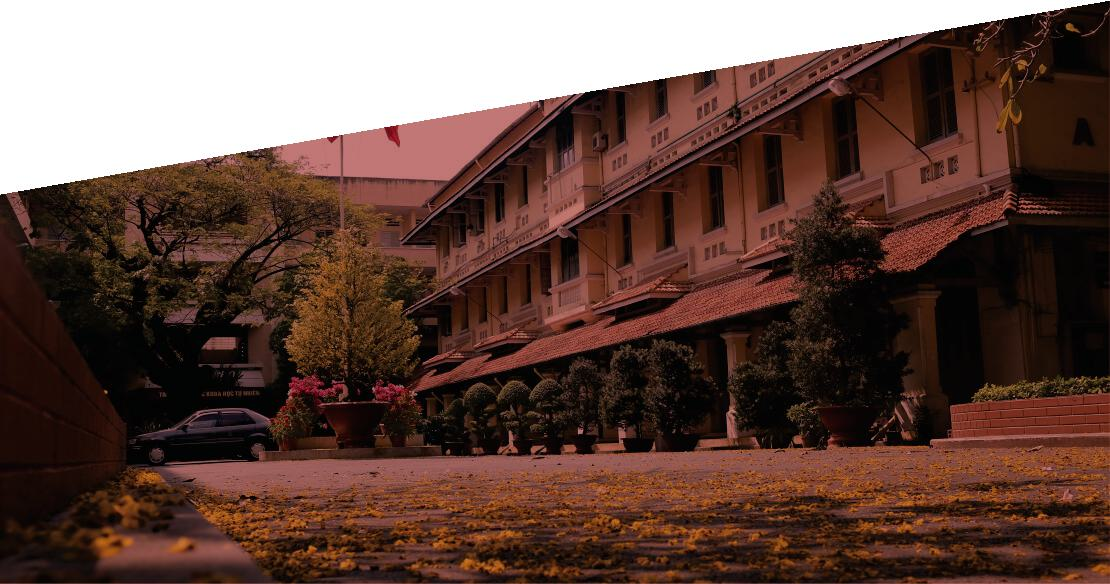
\includegraphics[width=\paperwidth]{Figures/0. General/fixed.jpeg}};

\mbox{}
\vfill
% \sffamily 
\Large \textcolor{white}{\normalfont \placeanddate} \\

\end{titlepage}









\newpage

% Table of Contents
\tableofcontents
\newpage

% need to update after all
\section{Preface}
This report is prepared for the Data Structures and Algorithms project by group 7 under the supervision of Mr. Nguyen Thanh Tinh. The work has been divided among team members, with their individual contributions outlined in the following table \ref{tab:work_assignment}:
\begin{table}[h!]
    \caption{Work assignment and contribution evaluation}
    \centering
    \begin{tabular}{|l|c|c|c|}
    \hline
    \textbf{Team Member} & \multicolumn{2}{|c|}{\textbf{Assigned Tasks}} & \textbf{Completion Rate (\%)}  \\ \hline
    \multirow{10}{*}{Thai Gia Huy} & \multirow{7}{*}{Report} & 1   & 100 \\ \cline{3-4}
                                  &                         & 2.2 & 100 \\ \cline{3-4}
                                  &                         & 3.3 & 100 \\ \cline{3-4}
                                  &                         & 4.2 & 100 \\ \cline{3-4}
                                  &                         & 5.3 & 100 \\ \cline{3-4}
                                  &                         & 6   & 100 \\ \cline{3-4}
                                  &                         & 8   & 100 \\ \cline{2-4}
                                  & \multirow{3}{*}{Slide}  & 3   & 100 \\ \cline{3-4}
                                  &                         & 4   & 100 \\ \cline{3-4}
                                  &                         & 5   & 100 \\ \cline{1-4}
    \multirow{9}{*}{Ho Thuy Tram} & \multirow{7}{*}{Report} & 2.1 & 100 \\ \cline{3-4}
                                  &                         & 3.1 & 100 \\ \cline{3-4}
                                  &                         & 3.2 & 100 \\ \cline{3-4}
                                  &                         & 4.1 & 100 \\ \cline{3-4}
                                  &                         & 5.1 & 100 \\ \cline{3-4}
                                  &                         & 5.2 & 100 \\ \cline{3-4}
                                  &                         & 7   & 100 \\ \cline{2-4}
                                  & \multirow{2}{*}{Slide}  & 1   & 100 \\ \cline{3-4}
                                  &                         & 2   & 100 \\ \cline{1-4}
    \end{tabular}
    
    \label{tab:work_assignment}
\end{table}

\vspace{10pt}

The report provides a comprehensive exploration of the LZW (Lempel-Ziv-Welch) compression algorithm, one of the most influential and widely used data compression techniques. The primary purpose of this report is to examine the theoretical foundations, practical applications, and performance characteristics of LZW, making it accessible to readers with an interest in data compression technologies.

\vspace{10pt}

The report begins with an introduction to the historical development of LZW and its significance in various real-world scenarios. It then delves into the algorithm's mechanics, outlining both the compression and decompression processes with illustrative examples to enhance understanding. Following this, the report analyzes the algorithm's performance, focusing on efficiency and how compression ratios influence time complexity. To place LZW in a broader context, the report provides an overview of related algorithms, such as LZ77 and LZ78, emphasizing their unique features and how they compare with LZW.
\vspace{10pt}

The report aims to offer a balanced view, covering both theoretical insights and practical implications. While every effort has been made to ensure the content is comprehensive and accurate, certain simplifications were adopted to maintain clarity and accessibility. Feedback and constructive suggestions for improvement are welcome as they will help refine this work further.
\newpage

\section{Introduction}
\subsection{Historical Background of LZW Compression}
Lempel-Ziv-Welch (LZW) is a widely known lossless, dictionary-based compression algorithm that builds upon the pioneering work of Abraham Lempel and Jacob Ziv on LZ78, published in 1978 in \textit{IEEE Transactions on Information Theory}\cite{doc1}. Terry Welch further refined the algorithm to improve its efficiency and adaptiveness, leading to his 1984 article, "A Technique for High-Performance Data Compression"\cite{doc2}, published in \textit{Computer}.

% \begin{figure}[htbp]
%     \centering
%     % 1st Image
%     \begin{subfigure}[b]{0.4\textwidth}
%         \centering
%         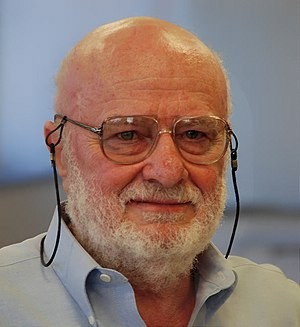
\includegraphics[width=\textwidth]{Figures/lempel.jpg}
%         \caption{Abraham Lempel}
%         \label{fig:lempel}
%     \end{subfigure}
%     \hfill
    
%     % 2nd image
%     \begin{subfigure}[b]{0.4\textwidth}
%         \centering
%         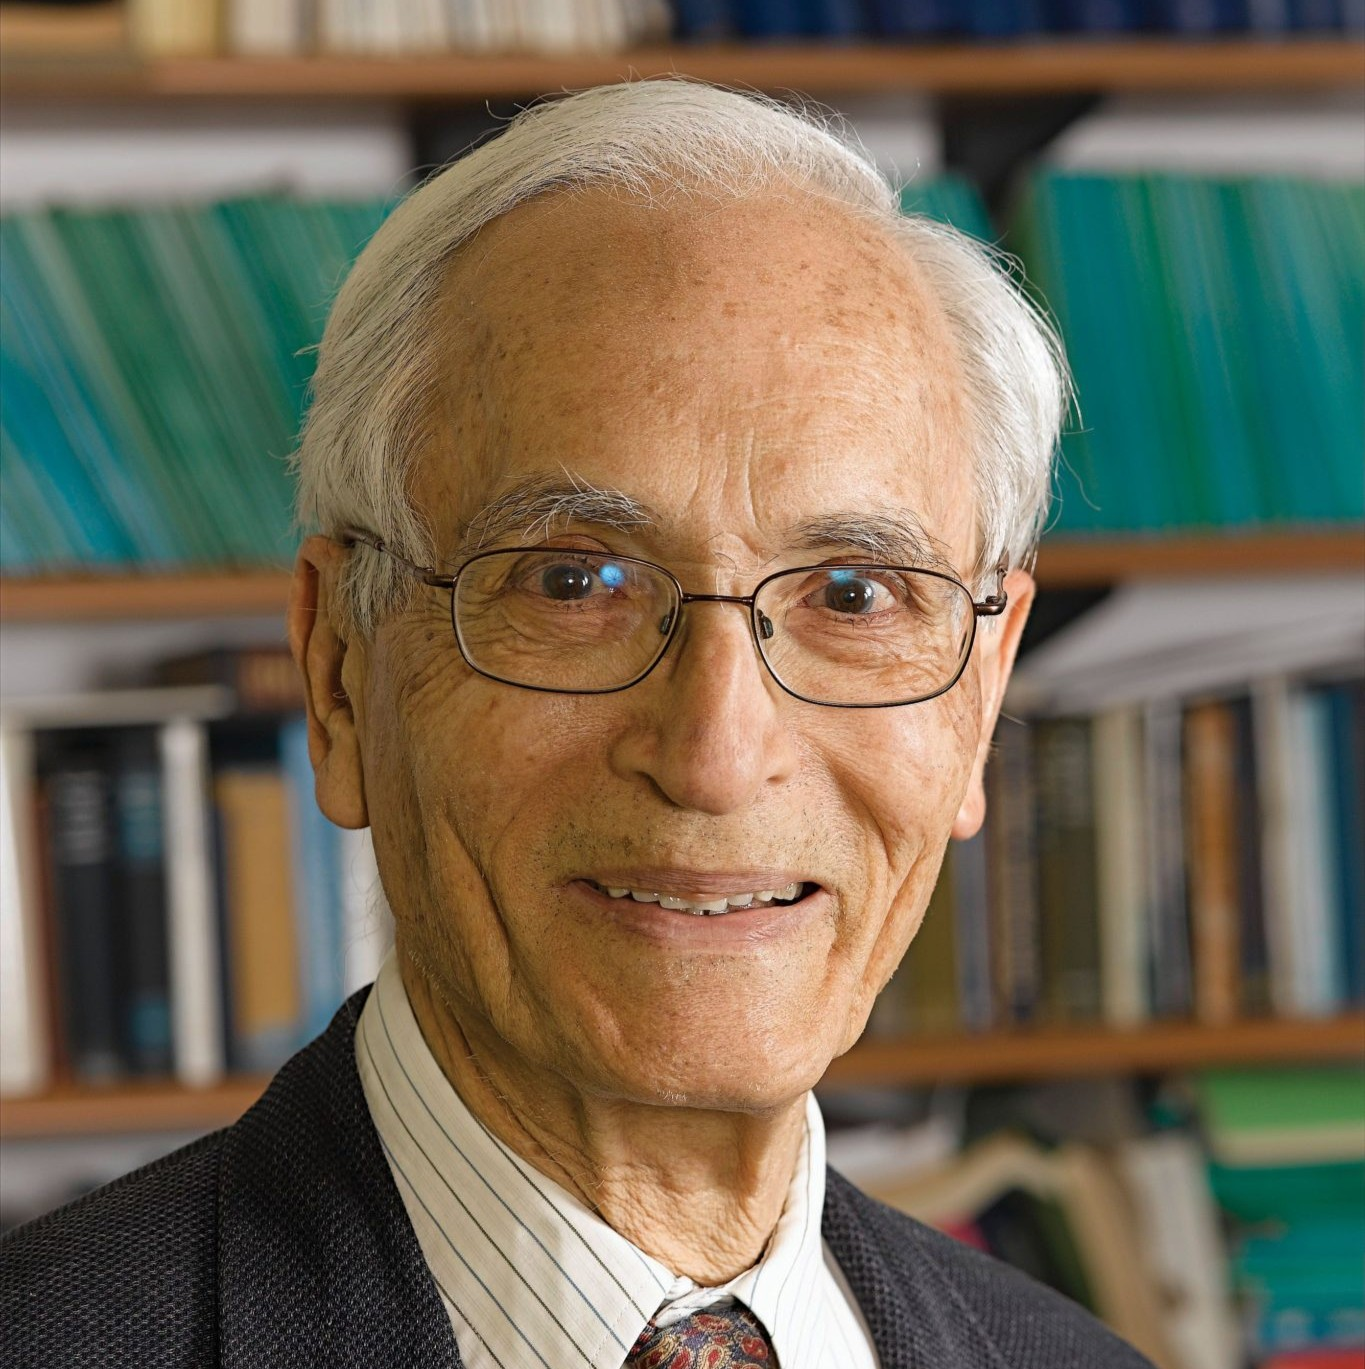
\includegraphics[width=\textwidth]{Figures/Ziv.jpeg}
%         \caption{Jacob Ziv}
%         \label{fig:ziv}
%     \end{subfigure}
    
%     \hfill
    
%     % 3rd image
%     \begin{subfigure}[b]{0.4\textwidth}
%         \centering
%         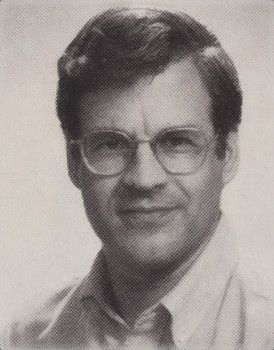
\includegraphics[width=\textwidth]{Figures/welch.jpg}
%         \caption{Terry Welch}
%         \label{fig:welch}
%     \end{subfigure}
%     \caption{Lempel - Ziv - Welch}
%     \label{fig:lzw}
% \end{figure}

% \begin{figure}[ht]
%  \centering
%  \begin{minipage}[b]{0.4\textwidth}
%   \centering
%   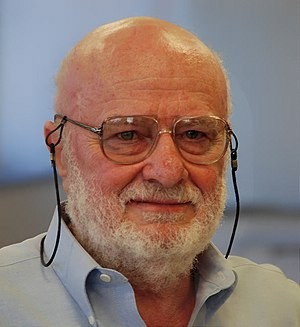
\includegraphics[height=0.85\textwidth]{Figures/lempel.jpg}
%   \caption{Abraham Lempel}
%  \end{minipage}%
%  \hfill
%  \begin{minipage}[b]{0.4\textwidth}
%   \centering
%   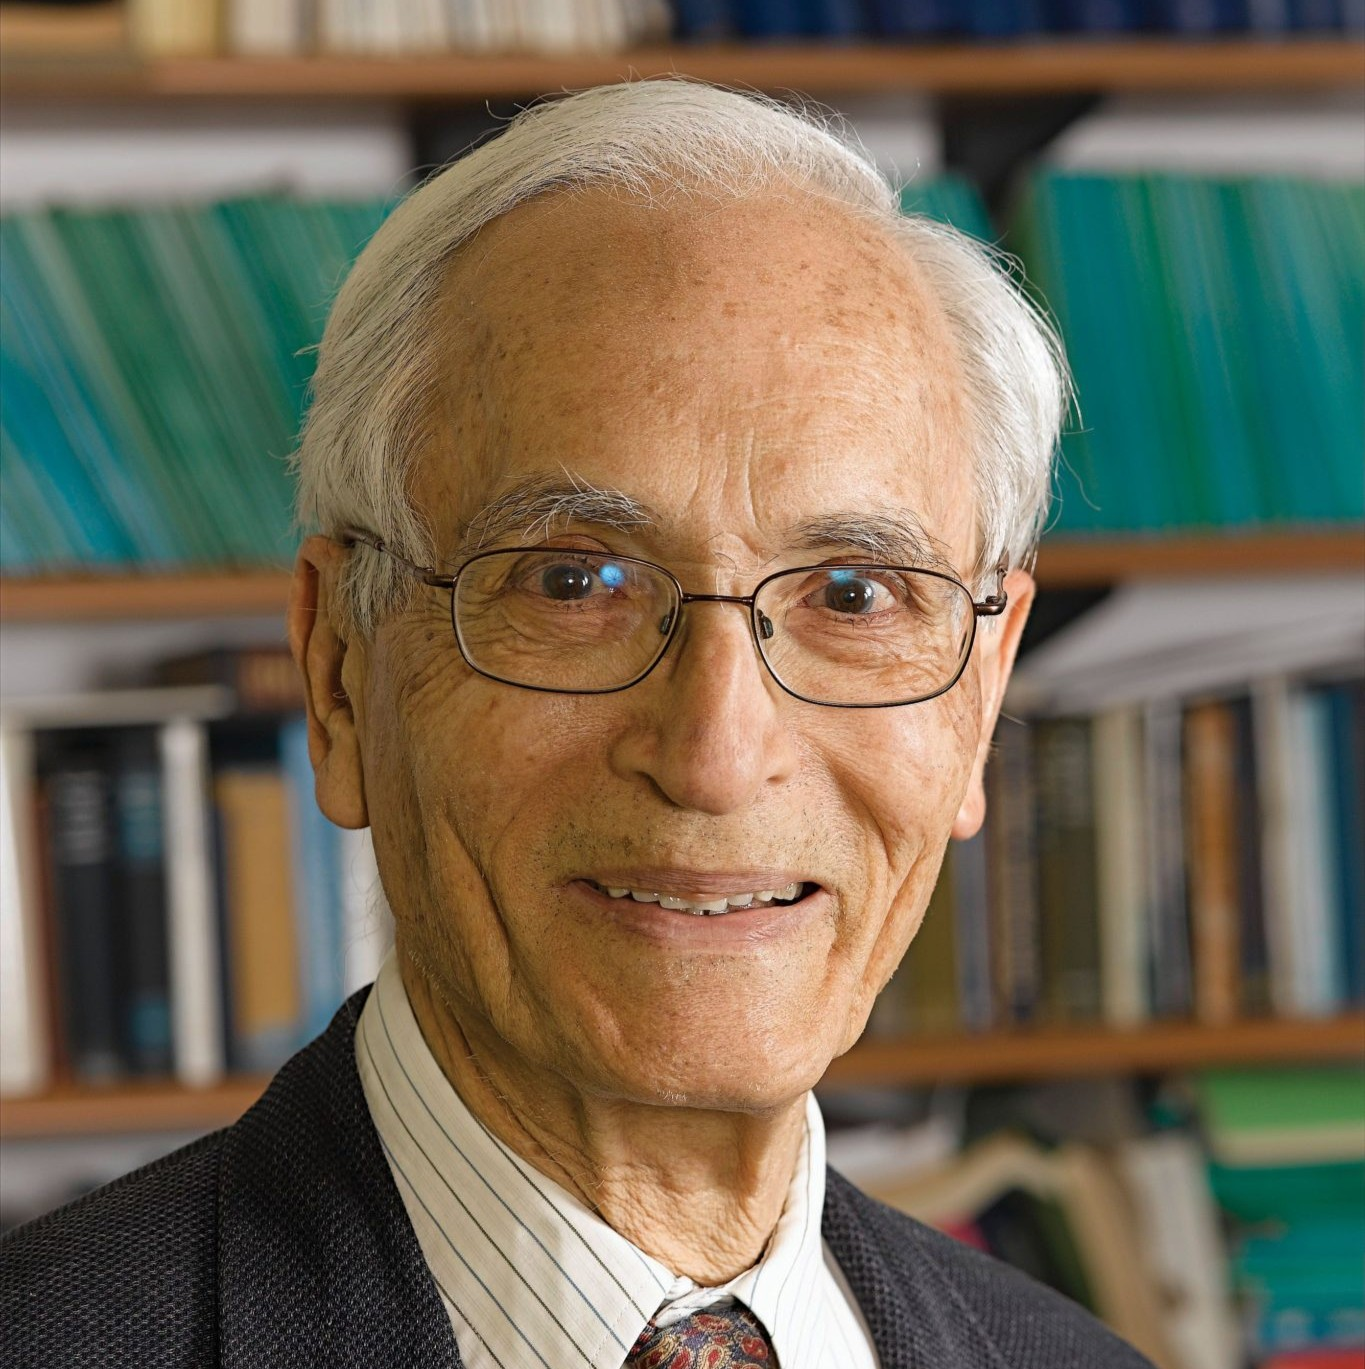
\includegraphics[height=0.85\textwidth]{Figures/Ziv.jpeg}
%   \caption{Jacob Ziv}
%  \end{minipage}

% \vskip\baselineskip
 
%  \begin{minipage}[b]{0.4\textwidth}
%   \centering
%   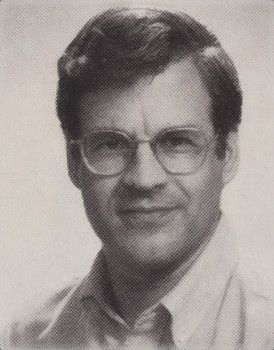
\includegraphics[height=0.85\textwidth]{Figures/welch.jpg}
%   \caption{Terry Welch}
%  \end{minipage}
% \end{figure}

\begin{figure}[ht]
    \centering
    \begin{minipage}{0.3\textwidth}
        \centering
        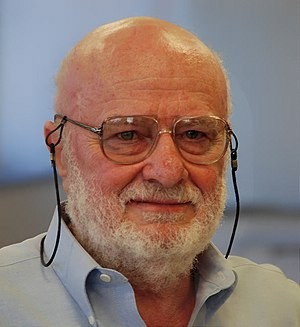
\includegraphics[width = \textwidth, height=1.1\textwidth]{Figures/lempel.jpg}
        \captionsetup{font=small}
        \caption{Abraham Lempel}
        \label{fig:fig1}
    \end{minipage}%
    \hfill
    \begin{minipage}{0.3\textwidth}
        \centering
        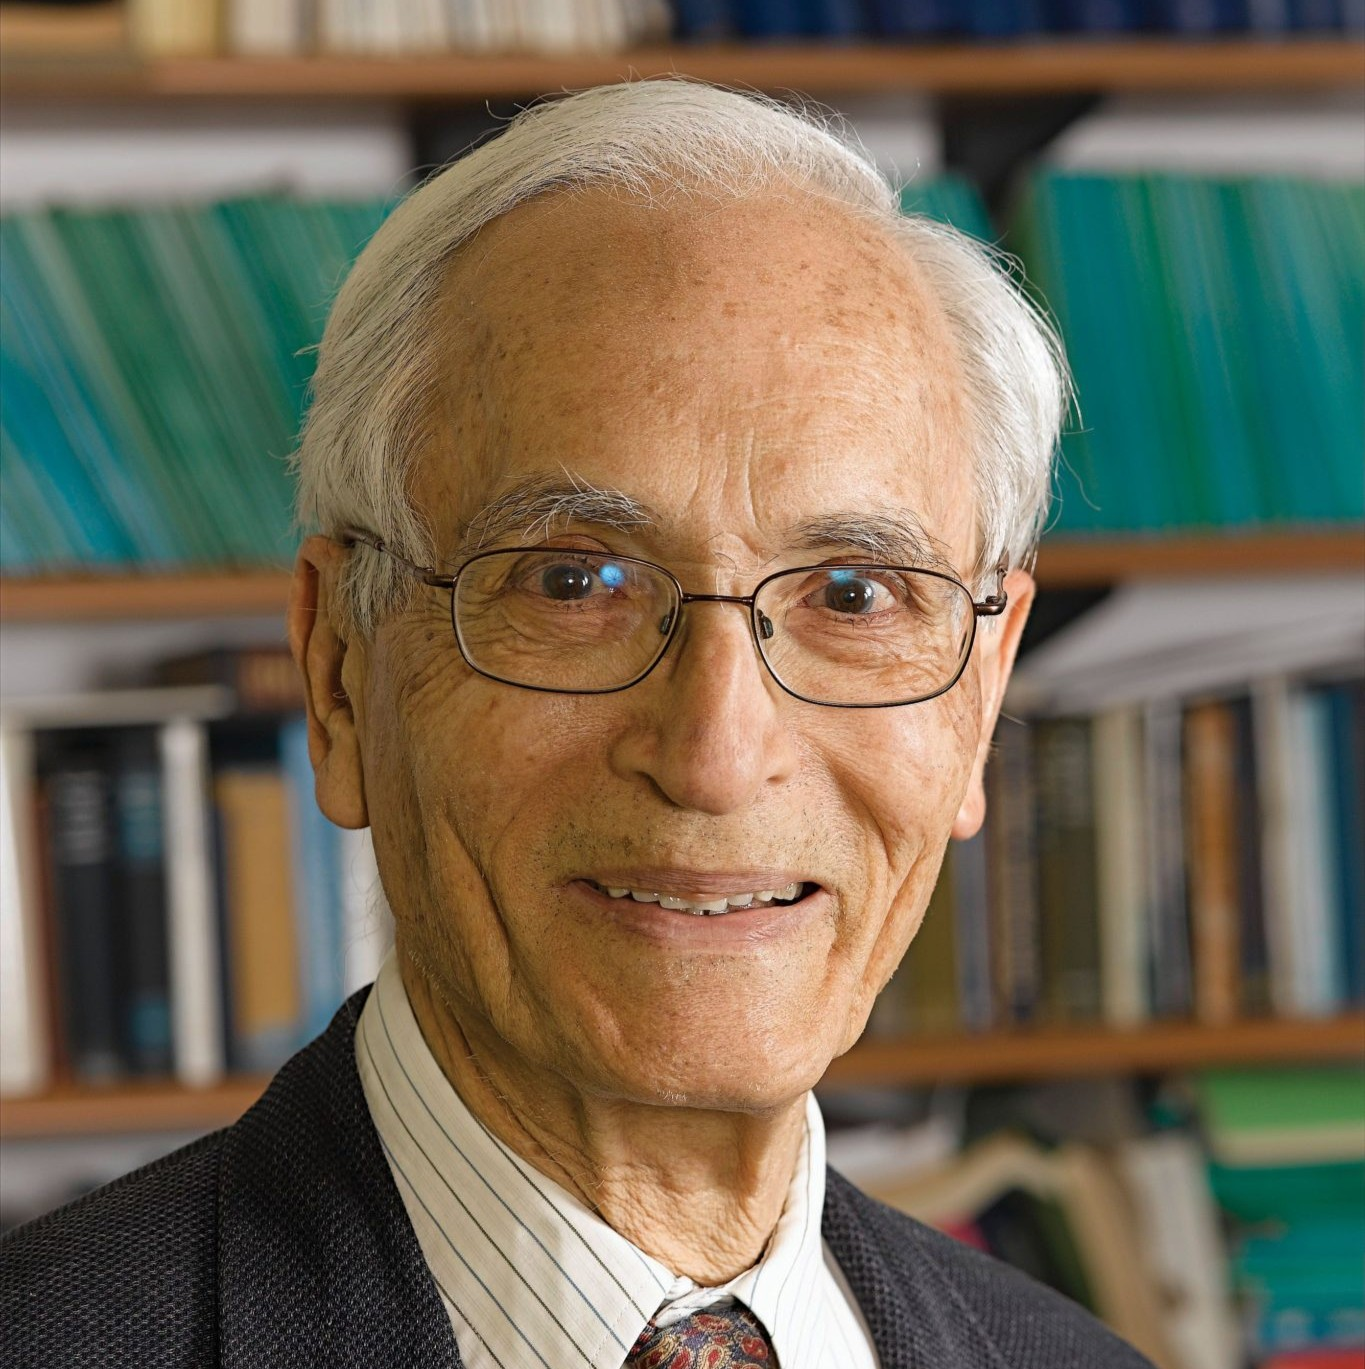
\includegraphics[width=\linewidth, height=1.1\textwidth]{Figures/Ziv.jpeg}
        \captionsetup{font=small}
        \caption{Jacob Ziv}
        \label{fig:fig2}
    \end{minipage}%
    \hfill
    \begin{minipage}{0.3\textwidth}
        \centering
        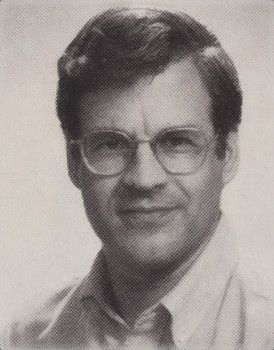
\includegraphics[width=\linewidth, height=1.1\textwidth]{Figures/welch.jpg}
        \captionsetup{font=small}
        \caption{Terry Welch}
        \label{fig:fig3}
    \end{minipage}
\end{figure}


The development of LZW arose from the need for efficient data compression methods during a time of rapidly growing digital information. Its design aimed to address the limitations of earlier compression methods by introducing a dynamic dictionary-based approach that did not require pre-analysis of the data. This adaptability marked a significant evolution in lossless compression techniques.

\vspace{10pt}

Unlike its predecessor LZ78, LZW uses a simplified mechanism to build and maintain its dictionary. This innovation made the algorithm computationally efficient and highly adaptable to various input data types, while preserving the core properties of the Lempel-Ziv methods. LZW's simplicity in logic allowed it to achieve high compression ratios without the complexity of earlier methods, making it a cornerstone in the history of data compression.
\subsection{Applications of LZW Compression}
\begin{figure}[ht]
    \centering
    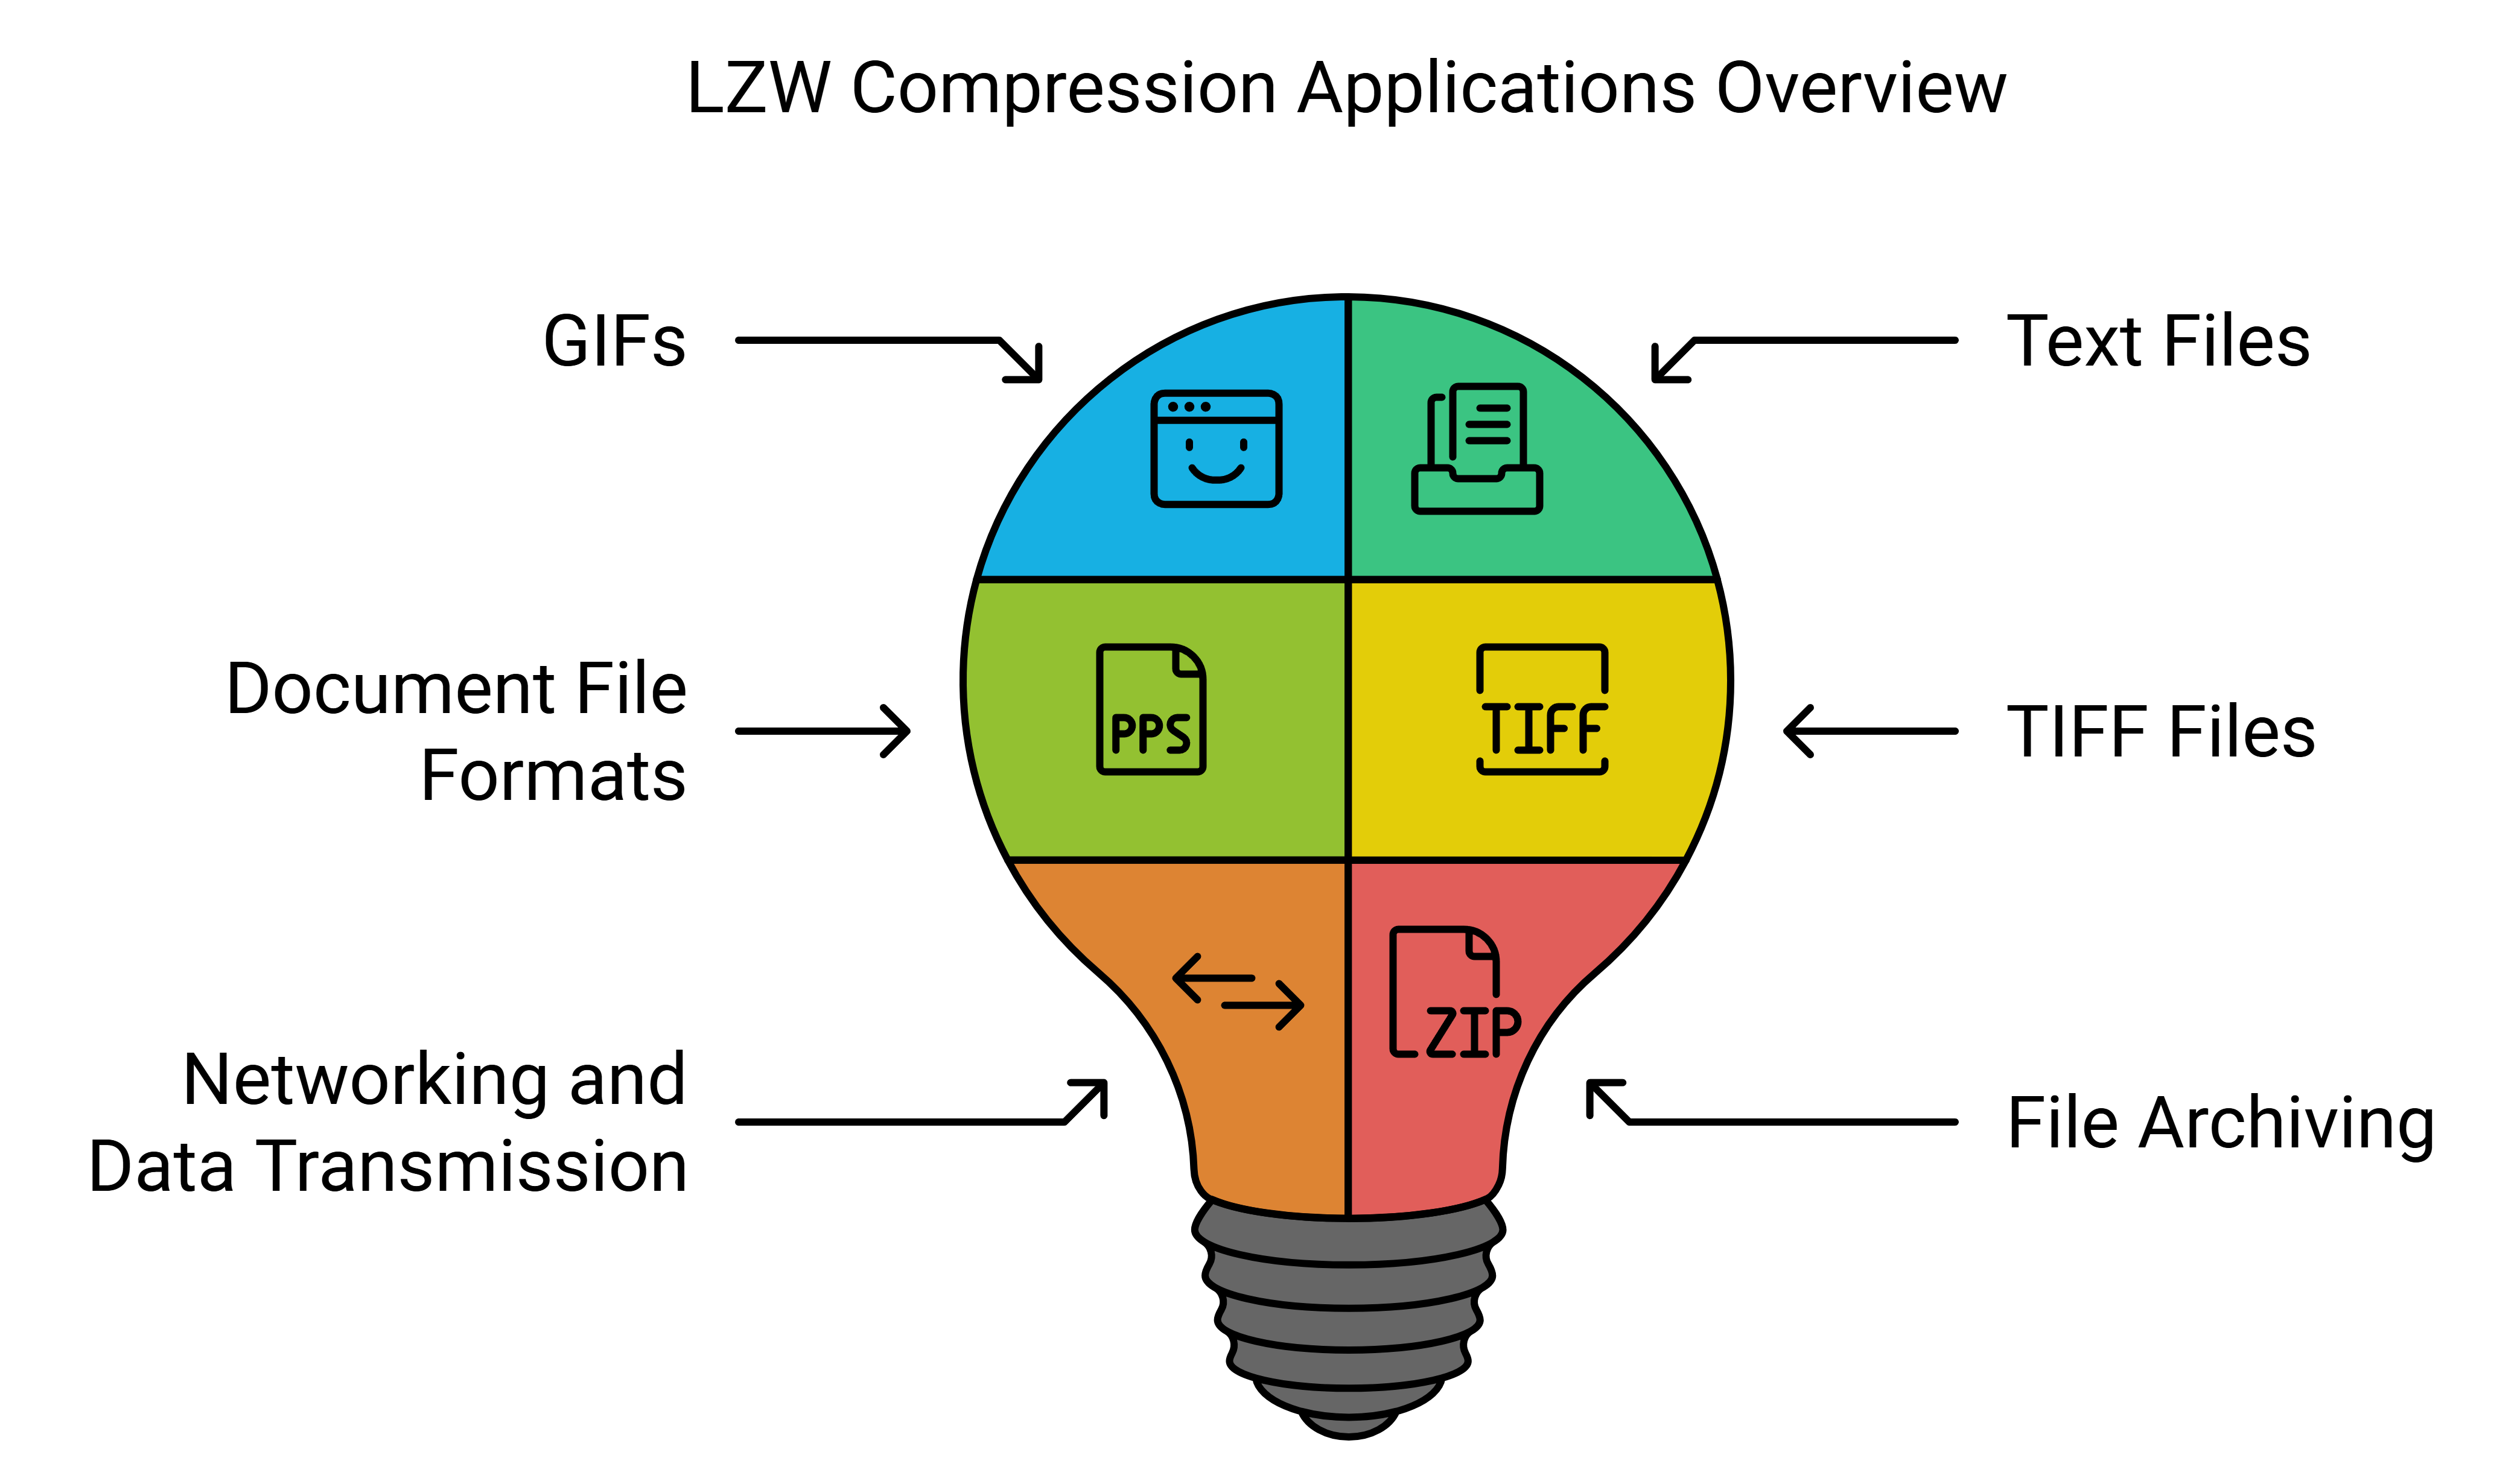
\includegraphics[width=0.8\linewidth]{Figures/application.png}
    \caption{Applications of LZW Compression}
\end{figure}

The LZW compression algorithm is a cornerstone of modern data compression, applied extensively due to its efficiency and reliability. One of its most recognizable applications is in the \textit{GIF (Graphics Interchange Format)}. GIFs utilize LZW compression to minimize file sizes while preserving image quality, enabling quick load times and low bandwidth usage, which are crucial for web graphics and animations.

\vspace{10pt}

In the domain of \textit{text compression}, LZW is highly effective for files with repetitive patterns, such as structured data in XML or JSON formats. By replacing repeating strings with shorter codes, the algorithm significantly reduces file sizes while retaining the ability to reconstruct the original content without any loss. This makes LZW indispensable in archiving and transferring text-based data.

\vspace{10pt}

LZW also plays a pivotal role in \textit{document file formats} like PostScript and PDF. These formats benefit from LZW's ability to optimize file sizes without compromising the integrity of the content, ensuring rapid rendering and efficient storage. This application is particularly valuable in professional publishing and document sharing.

\vspace{10pt}

In addition to GIFs, LZW is used in certain \textit{TIFF (Tagged Image File Format)} files. This is particularly relevant in medical imaging and archival photography, where maintaining high precision is essential. The lossless compression provided by LZW ensures that the quality and integrity of these critical files remain intact.
\vspace{10pt}

LZW's impact extends to \textit{networking and data transmission}. By compressing data before sending it, the algorithm reduces bandwidth requirements and accelerates transfer speeds, making it integral to systems that rely on high-speed communication and efficient resource usage.

\vspace{10pt}

Finally, the influence of LZW can be seen in \textit{file archiving and software packaging tools}. Formats like ZIP have drawn inspiration from LZW’s principles to enable efficient storage and transfer of large datasets and software installations. This reliability and effectiveness in handling large volumes of data have made LZW a foundational component in these technologies.

\vspace{10pt}

These examples demonstrate LZW’s versatility and its ability to address diverse needs, from compressing multimedia files to enhancing network efficiency. The algorithm’s continued relevance is a testament to its robustness and adaptability in modern computing.

\newpage

\section{Understanding the LZW Compression Algorithm}
\subsection{Key Concepts and Mechanisms}
Lempel-Ziv Welch coding makes use of dictionaries to store substrings of characters that have occured before in the text, thus "memorizing" them. When a repeating substring is recognized, it uses the indices of the place in the dictionary where the required substring is stored and compresses the text doing so. This method thus relies heavily on repetition. 

\vspace{10pt}
A further property is that it makes use of the "greedy" parsing algorithm, where the text is looped over exactly once. During this parsing, the longest recognized substring is saved to the result and the combination of the current substring and the next occurring character is added to the dictionary.

\vspace{10pt}
Since the dynamic dictionary is created by both compressor and decompressor with small dictionary of all possible single-character strings like ASCII characters, there is no dictionary transmission which reduces transmission overhead. 

\vspace{10pt}
Although this algorithm can achieve great compression, it does not attempt to optimally select strings by making use of probability estimation. Therefore, its effectiveness is less than optimal, but creates great usability by the simplicity of the algorithm.


\subsection{Compression Process with Examples}
% LZW Compression Process
\begin{algorithm}[H]
	\caption{LZW Compression Process} 
	\begin{algorithmic}[1]
\State Initialize an empty dictionary.
\State Populate the emptied dictionary with all possible one-length characters from the extended ASCII set (values 0 to 255).
\State Initialize an empty string $\mathbf{P}$.

\While{not at the end of the character stream}
    \State $\mathbf{C = \text{next character}}$.
    \If{$\mathbf{P + C}$ exists in the dictionary}
        \State $\mathbf{P = P + C}$ (Extend by adding C to the string P).
    \Else
        \State Output the code for $\mathbf{P}$.
        \State Append the string $\mathbf{P + C}$ to the dictionary.
        \State $\mathbf{P = C}$ (Replace the string P with the current character).
    \EndIf
\EndWhile
	\end{algorithmic} 
\end{algorithm}

\vspace{10pt}

The compression phase of the LZW algorithm involves scanning through the input data, identifying repeating sequences, and replacing them with shorter codes that refer to these sequences. Initially, the dictionary contains all possible individual symbols that appear in the input data. As the algorithm processes the input, it builds the dictionary dynamically by adding longer sequences of characters encountered during the scan.

\vspace{10pt}

The process starts by taking an input string and checking if it already exists in the dictionary. If the sequence is found, it is replaced with the corresponding code. If the sequence is not found, it is added to the dictionary with a new code, and the algorithm continues with the next symbol. This approach works efficiently when dealing with data that contains a lot of repetitive sequences, as a single code can replace each repeating pattern.

\vspace{10pt}

\textcolor{magenta}{\textbf{Example:}} LZW compression process for the string "\textcolor{Tue-red}{\textbf{ABCBCCAB}}".

\vspace{10pt}

\textbf{Initialize:} Dictionary with all possible single-length characters from the extended ASCII table. Each character serves as the key, and the corresponding value is initialized to 0, for instance: dictionary["0"] = 176, dictionary["A"] = 193.

% \begin{figure}[ht]
%   \centering
%   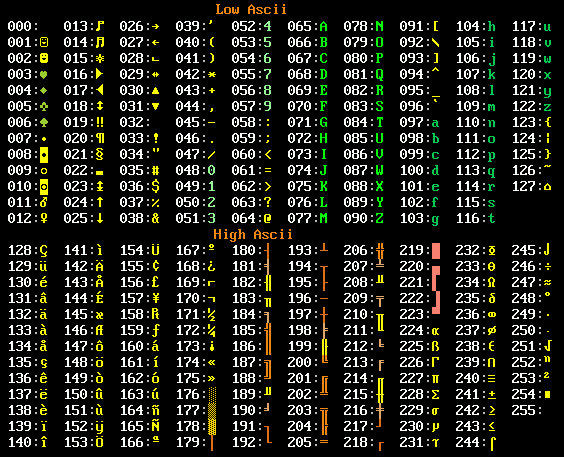
\includegraphics[height=0.5\textwidth]{Figures/ascii.png}
%   % \caption{extended ASCII set}
% \end{figure}

\begin{table}[ht]
    \caption{Trace of the LZW Algorithm step by step: Compression process}
    \centering
\adjustbox{max width=\textwidth}{
\begin{tabular}{|c|c|c|c|c|l|}
\hline
\multirow{2}{*}{\textbf{Step}} & \multicolumn{2}{|c|}{\textbf{Encoder Output}} & \multicolumn{2}{c|}{\textbf{Dictionary}} & \multirow{2}{*}{\textbf{Explaination}} \\ \cline{2-5}
 & \textbf{Output} & \textbf{Represents} & \textbf{Key} & \textbf{Value} & \\ \hline
1 &  &  &  &  & P = "", C = "A", assign P+C = "A" to P \\ \hline
2 & 193 & "A" & "AB" & 256 & P = "A", C = "B",  assign C = "B" to P\\ \hline
3 & 194 & "B" & "BC" & 257 & P = "B", C = "C", assign C = "C" to P \\ \hline
4 & 195 & "C" & "CB" & 258 & P = "C", C = "B", assign C = "B" to P \\ \hline
5 &  &  &  &  & P = "B", C = "C", assign P+C = "BC" to P \\ \hline
6 &  257& "BC" & "BCC" & 259 & P = "BC", C = "C", assign C = "C" to P \\ \hline
7 & 195 & "C" & "CA" & 260 & P = "C", C = "A", assign C = "A" to P \\ \hline
8 &  &  &  &  & P = "A", C = "B", assign P+C = "AB" to P \\ \hline
9 & 256 & "AB" &  &  & P = "AB", C = ""\\ \hline
&   &   &  & & end of stream \\ \hline
\end{tabular}
}

    \label{tab:lzw_trace_compress}
\end{table}

\textbf{Encoder:} The compressor output is the binary form of each column encoder output for characters representation, such as here: \textbf{\textcolor{cyan}{193 194 195 257 195 256}}.





\subsection{Decompression Process with Examples}
% LZW Decompression Process
\begin{algorithm}[H]
	\caption{LZW Decompression Process} 
	\begin{algorithmic}[1]
        \State Initialize the dictionary with all possible single-length characters.
        \State $\textbf{OLD}$ = first input code.
        \State Output translation of $\textbf{OLD}$ (decoded sequence).
        
        \While{not at the end of the encoded sequence}
            \State $\textbf{NEW}$ = next input code.
            \If{$\textbf{NEW}$ exists in the dictionary}
                \State $S$ = translation of $\textbf{NEW}$.
            \Else
                \State $S$ = translation of $ \textbf{OLD}$ + $C$.
            \EndIf
            \State Output $S$.
            \State $C$ = first character of $S$.
            \State Append translation of $\textbf{OLD}$ + $C$ to the dictionary.
            \State $\textbf{OLD}$ = $\textbf{NEW}$.
        \EndWhile
	\end{algorithmic} 
\end{algorithm}

\vspace{10pt}

The decompression phase of the LZW algorithm is designed to reverse the compression process, reconstructing the original data from the compressed codes. The decompression algorithm begins with the same initial dictionary used during the compression phase, containing all individual symbols. It then reads the compressed data, consisting of a series of codes referencing sequences in the dictionary.

\vspace{10pt}

As the decompressor processes each code, it retrieves the corresponding sequence from the dictionary and adds it to the output. If the code refers to an existing sequence, the sequence is output directly. If the code refers to a new sequence, the decompressor will add the sequence to the dictionary, ensuring it can be used in subsequent decompression steps.

\vspace{10pt}
\textcolor{magenta}{\textbf{Example:}} LZW decompression process for the encoded input \textcolor{cyan}{193 194 195 257 195 256}.\\ \\
\textbf{Initialize:} Dictionary with all possible single-length characters, mapping ASCII character codes, for instance: dictionary[176] = "0", dictionary[193] = "A".

\begin{table}[ht]
    \caption{Trace of the LZW Algorithm step by step: Decompression process}
    \centering
\adjustbox{max width=\textwidth}{
\begin{tabular}{|c|c|c|c|l|}
\hline
\multirow{2}{*}{\textbf{Step}} & \multirow{2}{*}{\textbf{Decoder Output}} & \multicolumn{2}{c|}{\textbf{Dictionary}} & \multirow{2}{*}{\textbf{Explaination}} \\ \cline{3-4}
& & \textbf{Key} & \textbf{Value} & \\ \hline
1 &  "A" &   &  &  OLD = 193\\ \hline
2 &  "B" &  256 & "AB" & NEW = 194, S = "B", C = "B", OLD = 194\\ \hline
3 &  "C" &  257 & "BC" & NEW = 195, S = "C", C = "C", OLD = 195 \\ \hline
4 &  "BC" & 258 & "CB" & NEW = 257, S = "BC", C = "B", OLD = 257 \\ \hline
5 &  "C" &  259 & "BCC" & NEW = 195, S = "C", C = "C", OLD = 195 \\ \hline
6 &  "AB" &  260 & "CA" & NEW = 256, S = "AB", C = "A", OLD = 256 \\ \hline
 &   &   &  & end of stream \\ \hline
\end{tabular}
}

    \label{tab:lzw_trace_decompress}
\end{table}

\textbf{Decocoder:} The decompressor output of encoded input is the string reconstructed from binary encoders, such as here: "\textbf{\textcolor{Tue-red}{ABCBCCAB}}".


\newpage

\section{Performance Analysis of LZW Compression}
\subsection{Compression Ratios}
% https://courses.cs.duke.edu/spring03/cps296.5/papers/welch_1984_technique_for.pdf
The effectiveness of compression is expressed as a ratio relating to the number of bits needed to express the message before and after compression. The compression ratio used here will be the uncompressed bit count divided by the compressed bit count. The resulting value, usually greater than one, indicates the factor of increased data density achieved by compression. 
For example, compression that serves to eliminate half the bits of a particular message is presented as fulfilling a 2.0 compression ratio, indicating that two-to-one compression has been achieved.

\vspace{10pt}
The compression ratios presented in the table below are derived from the original article "A Technique for High-Performance Data Compression"\cite{doc2} by Terry Welch. These results, obtained through software simulation, are provided in Table \ref{tab:compression_results} for various data types.

\begin{table}[h!]
\caption{Compression results for a variety of data types.}
\centering
\begin{tabular}{|l|c|}
\hline
\textbf{Data Type}               & \textbf{Compression Ratio} \\ \hline
English Text                     & 1.8                        \\ \hline
Cobol Files                      & 2 to 6                     \\ \hline
Floating Point Arrays            & 1.0                        \\ \hline
Formatted Scientific Data        & 2.1                        \\ \hline
System Log Data                  & 2.6                        \\ \hline
Program Source Code              & 2.3                        \\ \hline
Object Code                      & 1.5                        \\ \hline
\end{tabular}
\label{tab:compression_results}
\end{table}


% Cobol Files, Formatted Scientific Data, System Log Data, Program Source Code

\textbf{English text.} Text samples for compression were obtained from ASCII word processing files in a technical environment. Results were reasonably consistent for simple text, at a compression ratio of 1.8. Surprisingly, long individual documents did not compress better than groups of short documents, indicating that other factors (such as formatting or structural information) might be contributing more significantly to redundancy, rather than the content itself.

\vspace{10pt}

\textbf{Cobol Files.} A significant number of large Cobol files from several types of applications were compressed, producing widely variable results. Compression depends on record format, homogeneity across data records, and the extent of integer usage. These were eight-bit ASCII files, so the integer data would compress very well. A side experiment showed that one-third to two-thirds of the space in some of these files appeared as strings of repeated identical characters, indicating a high fraction of blank space (fixed-width record format).

\vspace{10pt}

\textbf{Floating Point Arrays.} Arrays of floating point numbers look pretty much like white noise and so they compress rather poorly. The fraction part is a nearly random bit pattern since there are no redundancy savings to offset the overhead.

\vspace{10pt}

\textbf{Formatted Scientific Data.} Most data used by Fortran programs tended to compress about 50 percent. This data included input data, primarily integers. It also included print files, which were ASCII-coded.

\vspace{10pt}

\textbf{System Log Data.} Information describing past system activity, such as job start and stop times, is mostly formatted integers and is therefore reasonably compressible. This log data is used for recovery and constitutes perhaps 10 percent of the data stored on backup/recovery tapes. It tends to be in a tightly packed, fixed-length format, so the compression achieved is due to null fields and repetition in the data values.


\vspace{10pt}

\textbf{Program Source Code.} Source code can be compressed by a factor of better than two. It can be compressed better than text because words are frequently repeated and blank spaces are introduced by the source code format. Highly structured programming yields source code with greater compressibility than the average 2.3 factor cited here.

\vspace{10pt}
\textbf{Object Code.} Object code consists of arbitrary bit patterns and does not compress well. Uneven usage of opcodes and incomplete utilization of displacement fields would account for most of the compression achieved.

\subsection{Time Complexity}
The performance of LZW compression is influenced by the type of input data being processed. Different data types often exhibit varying compression ratios, as the efficiency of the algorithm depends on the frequency and patterns of repeating sequences within the input. For example, highly repetitive data tends to achieve better compression ratios, thereby reducing the computational workload per unit of compressed output. Conversely, inputs with little to no redundancy may lead to lower compression ratios and potentially increase the time required for dictionary operations. This relationship between data characteristics and compression efficiency underscores the need to evaluate LZW’s performance under diverse data scenarios.

\vspace{10pt}

% for English Text
When applied to English text, the complexity depends on the structure of the input. We will explore both the Best Case and Worst Case scenarios, supported by mathematical reasoning. Additionally, as the dictionary grows, operations like searching and updating may become more computationally expensive, which can further affect performance in scenarios with large or non-repetitive datasets.

\vspace{10pt}

\subsubsection{Best Case}
The best-case scenario for LZW compression occurs when the input data exhibit highly repetitive patterns, allowing the algorithm to use its dictionary efficiently. For example, an input like \textit{"aaaaaaa"} or \textit{"abababab"} is ideal. In this case:

\begin{itemize}
    \item After the initial iterations, most substrings encountered in the input are already present in the dictionary. The algorithm quickly matches these patterns with existing dictionary entries, minimizing the need for new insertions. Each search operation is $\mathcal{O}(1)$ on average when using a hash table for the dictionary.
    \item Since the input is repetitive, new entries are rarely added to the dictionary. As a result, the dictionary remains small, reducing memory usage and processing overhead. This efficient usage of the dictionary further enhances performance.
    \item The compression process involves scanning through the input and performing a constant-time dictionary lookup for each character. The overall complexity is $\mathcal{O}(L)$, where $L$ is the length of the input. The decompression process follows a similar pattern, as most patterns are reused, and the dictionary's small size ensures fast lookups. Thus, the complexity is $\mathcal{O}(L_c)$, where $L_c$ is the compressed data length.
\end{itemize}

\vspace{10pt}

The chart below displays the results of several test cases, each containing a string with repetitive patterns of varying lengths:

\begin{figure}[ht]
    \centering
    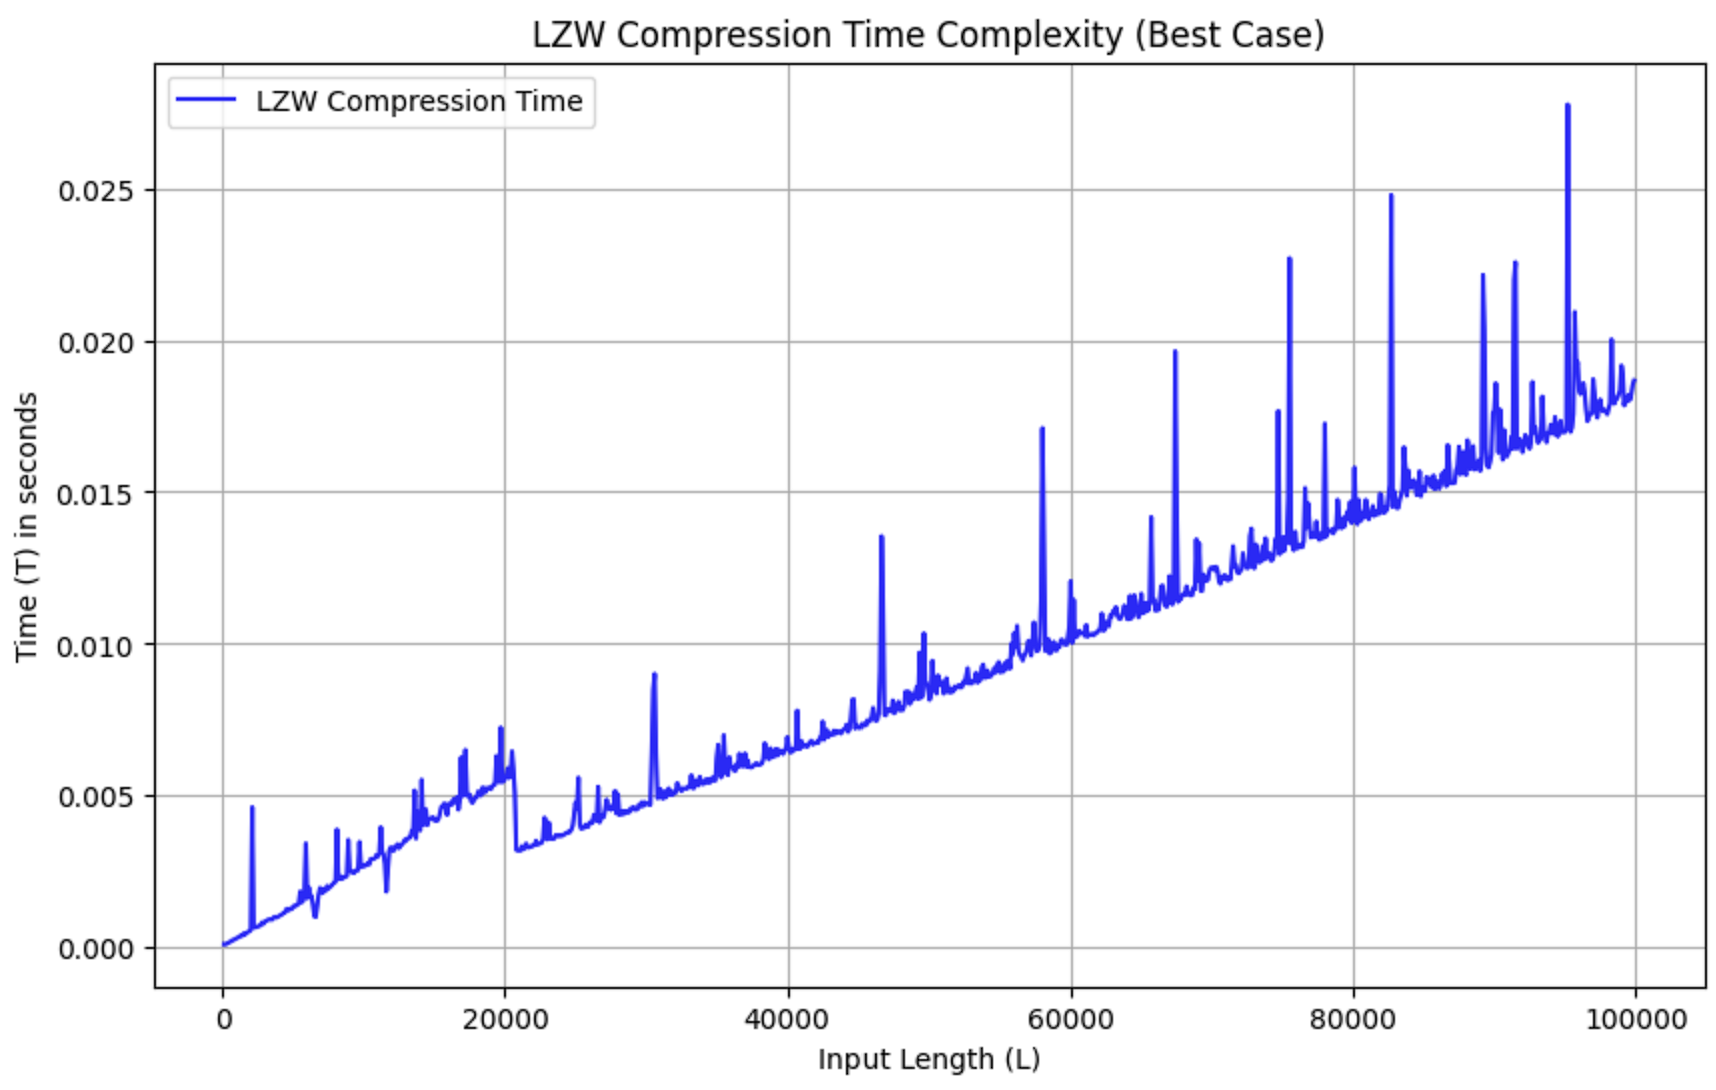
\includegraphics[width=0.8\linewidth]{Figures/best_case.png}
    \caption{LZW Compression Runtime in Best Case}
    \label{fig:bestcase}
\end{figure}

Based on this, we can prove that $T = \mathcal{O}(L)$ using the following chart:

\begin{figure}[ht]
    \centering
    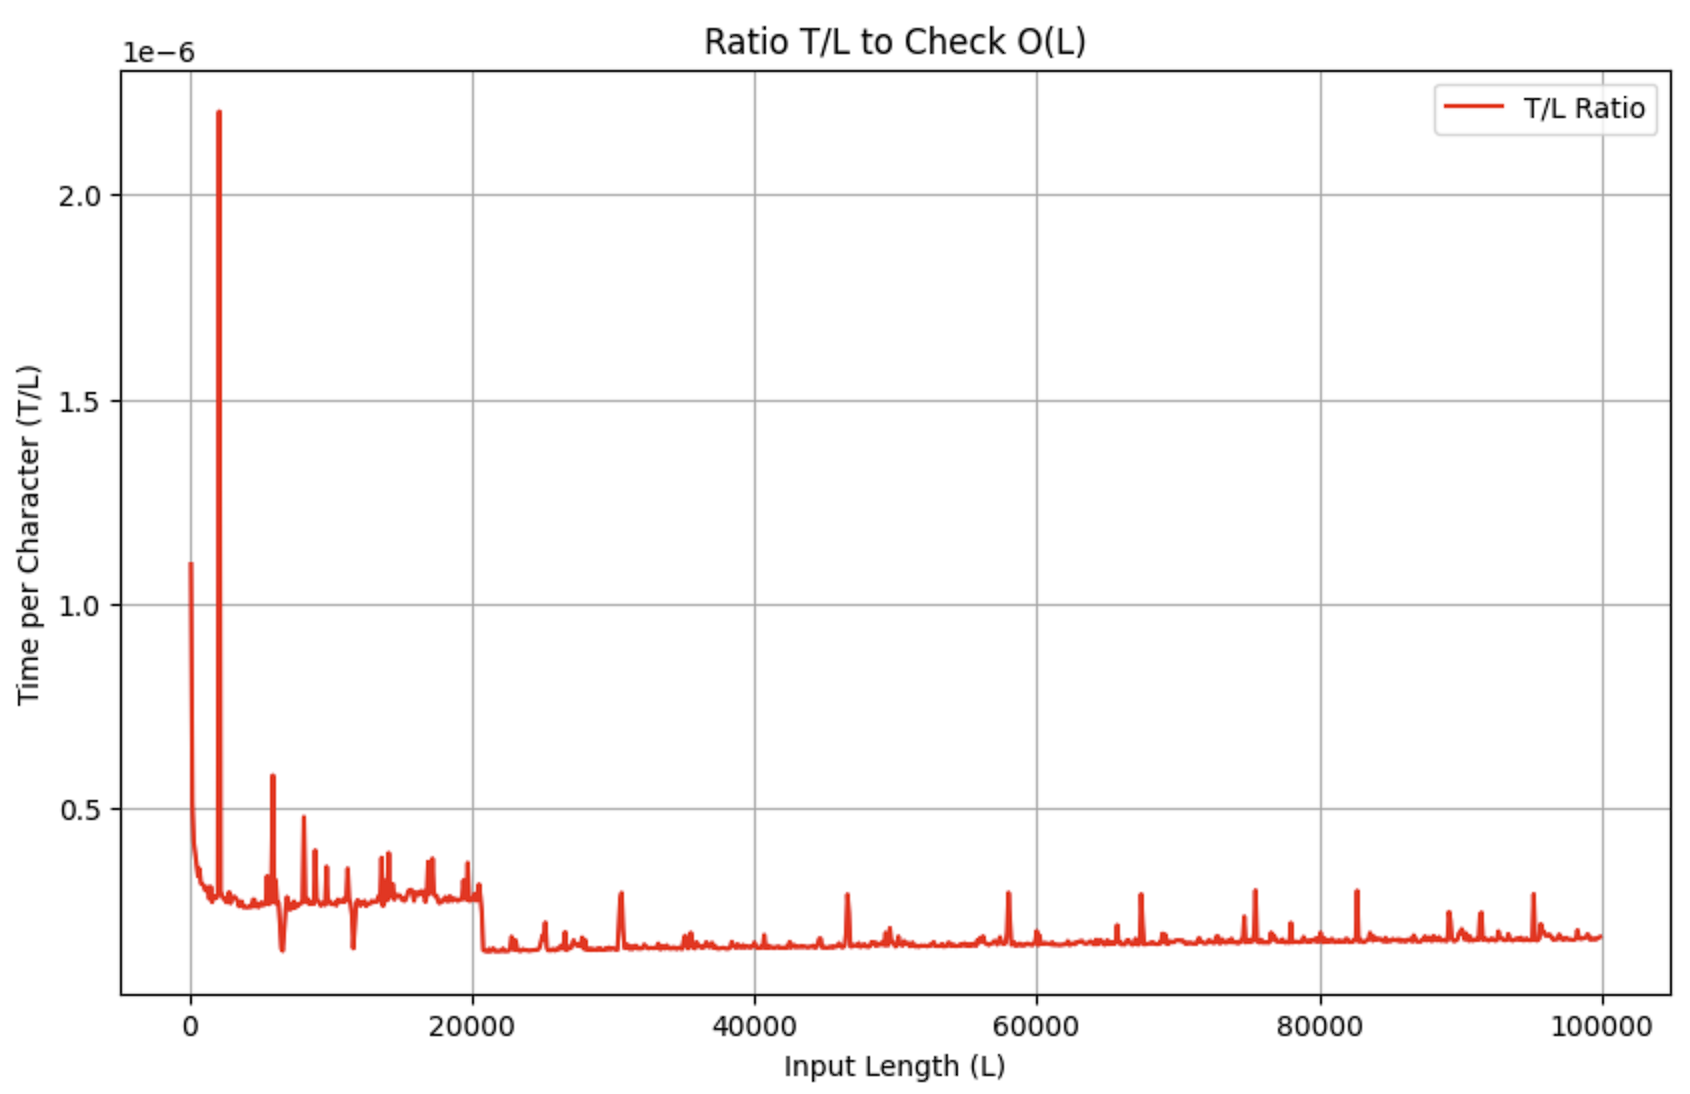
\includegraphics[width=0.8\linewidth]{Figures/bestcase_prove.png}
    \caption{Best Case: $T = \mathcal{O}(L)$}
    \label{fig:enter-label}
\end{figure}

\newpage

\subsubsection{Worst Case}
The worst-case scenario for LZW compression arises when the input data lacks any repetition or structure, such as unique or random characters. For example, an input like "abcdefg..." forces the algorithm to handle every substring as a new entity. In this case:

\begin{itemize}
    \item Every substring encountered in the input is unique and not found in the dictionary. This means that the algorithm frequently needs to perform dictionary insertions. Although lookups are $\mathcal{O}(1)$ on average, the frequent insertions can cause the dictionary size to grow rapidly.
    \item With each new substring, the dictionary expands, potentially reaching its maximum size $M$ quickly. If the dictionary size is not capped, this continuous growth consumes more memory and may degrade performance. In cases where a dictionary cap is implemented, frequent resets or replacements add additional overhead.
    \item Compression and decompression in the worst case are heavily affected by the rapid growth of the dictionary. Each character or code requires a dictionary lookup, and most substrings demand insertions. While the average-case lookup complexity remains $\mathcal{O}(1)$ with hash tables, poor hash distributions or collisions can degrade lookup performance to $\mathcal{O}(M)$, where $M$ is the dictionary size. Consequently, the compression complexity can reach $\mathcal{O}(L \cdot M)$, and the decompression complexity can grow to $\mathcal{O}(L_c \cdot M)$, where $L, L_c$ are the input and compressed lengths, respectively.
\end{itemize}

\vspace{10pt}

The following chart presents the results of multiple test cases, each containing a random string (barely repetitive) of different lengths:

\begin{figure}[ht]
    \centering
    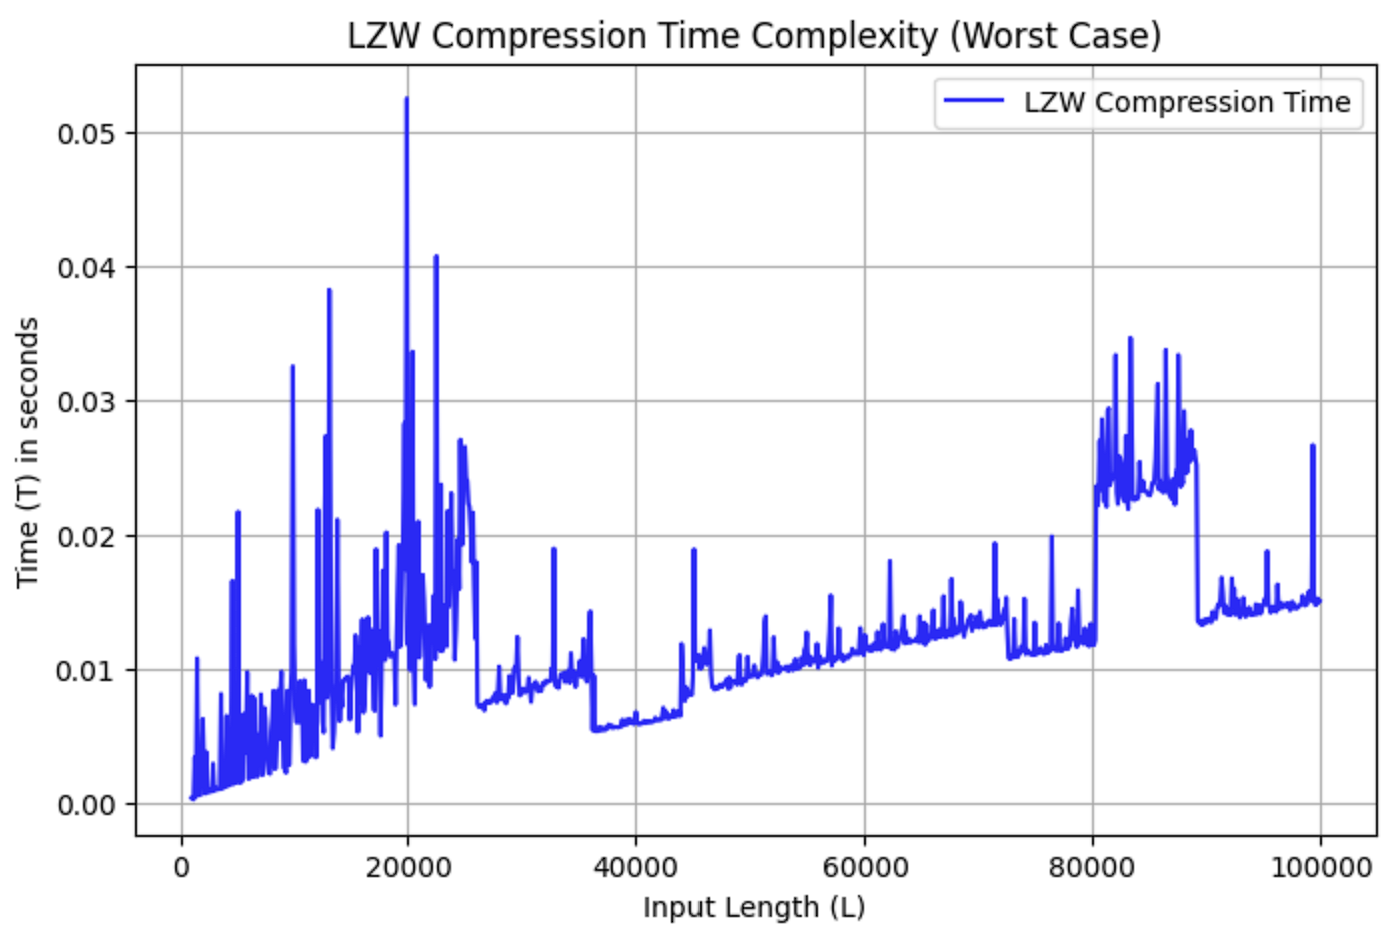
\includegraphics[width=0.8\linewidth]{Figures/worst_case.png}
    \caption{LZW Compression Runtime in Worst Case}
    \label{fig:worstcase}
\end{figure}

\newpage

From this, we can demonstrate that $T = \mathcal{O}(L \cdot M)$  through the following chart:

\begin{figure}[ht]
    \centering
    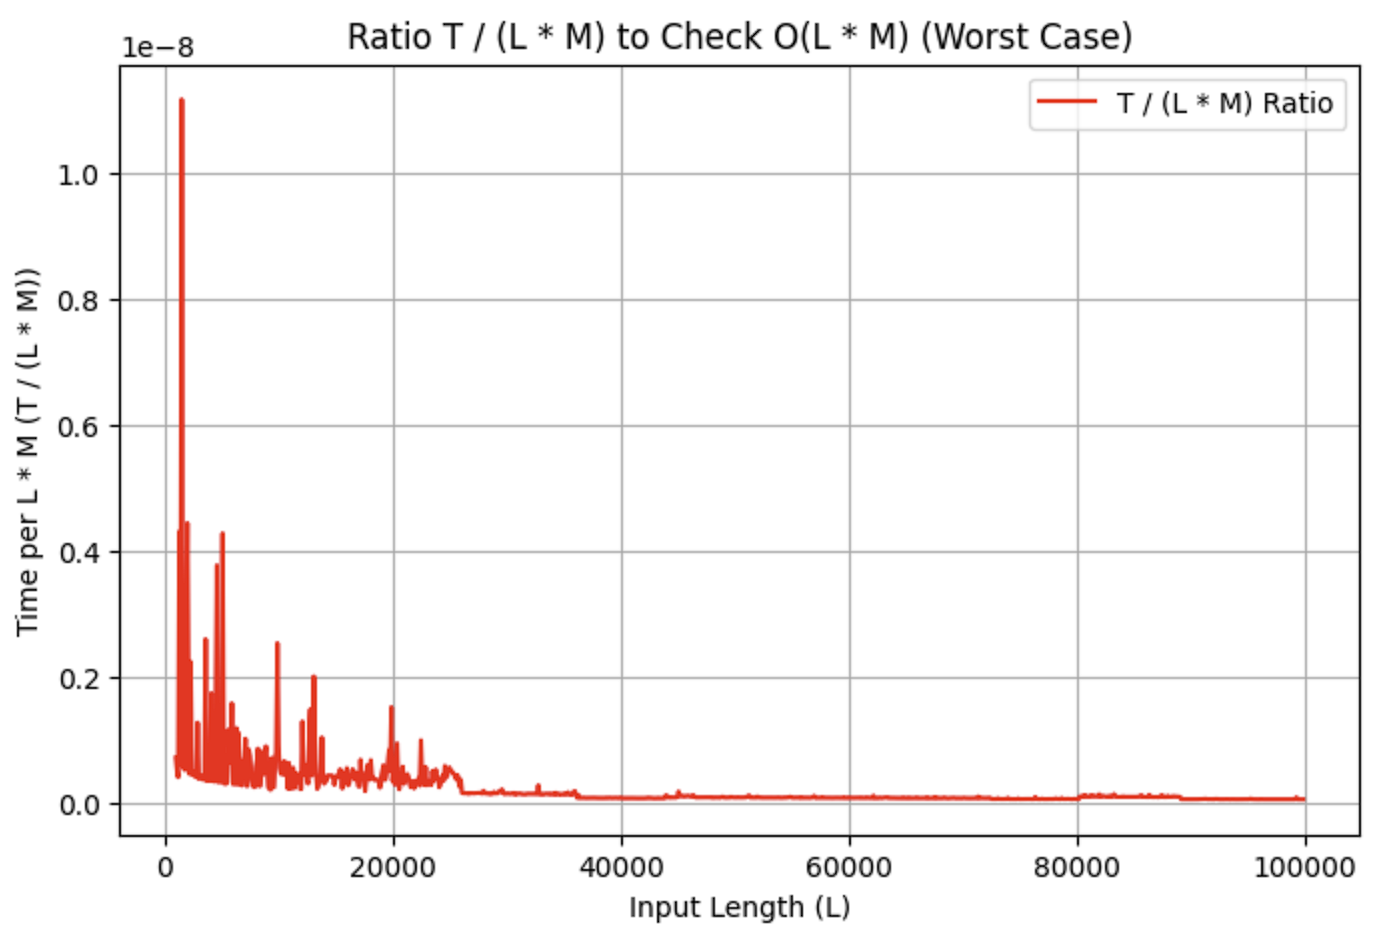
\includegraphics[width=0.8\linewidth]{Figures/worstcase_prove.png}
    \caption{Worst Case: $T = \mathcal{O}(L \cdot M)$}
    \label{fig:prove_worstcase}
\end{figure}
\newpage

\section{Overview of LZW-Related Algorithms}
LZ77 and LZ78 are the two most common lossless data compression algorithms, which Abraham Lempel and Jacob Ziv published in 1977\cite{doc3} and 1978 \cite{doc1}. They are sometimes referred to as LZ1 and LZ2 respectively. These two theoretical dictionary algorithms form the basis for many variations including LZW, LZSS, and others. Additionally, they are also the basis of several ubiquitous compression schemes, including GIF and the DEFLATE algorithm used in PNG.

\subsection{LZ77}
% https://en.wikipedia.org/wiki/LZ77_and_LZ78
LZ77\cite{doc4} operates on the concept of a sliding window, which tracks a portion of previously processed data. The algorithm identifies the longest match between a substring in the look-ahead buffer and a substring within the sliding window. After locating a match, the window slides forward based on the length of the match.

\begin{figure}[ht]
    \centering
    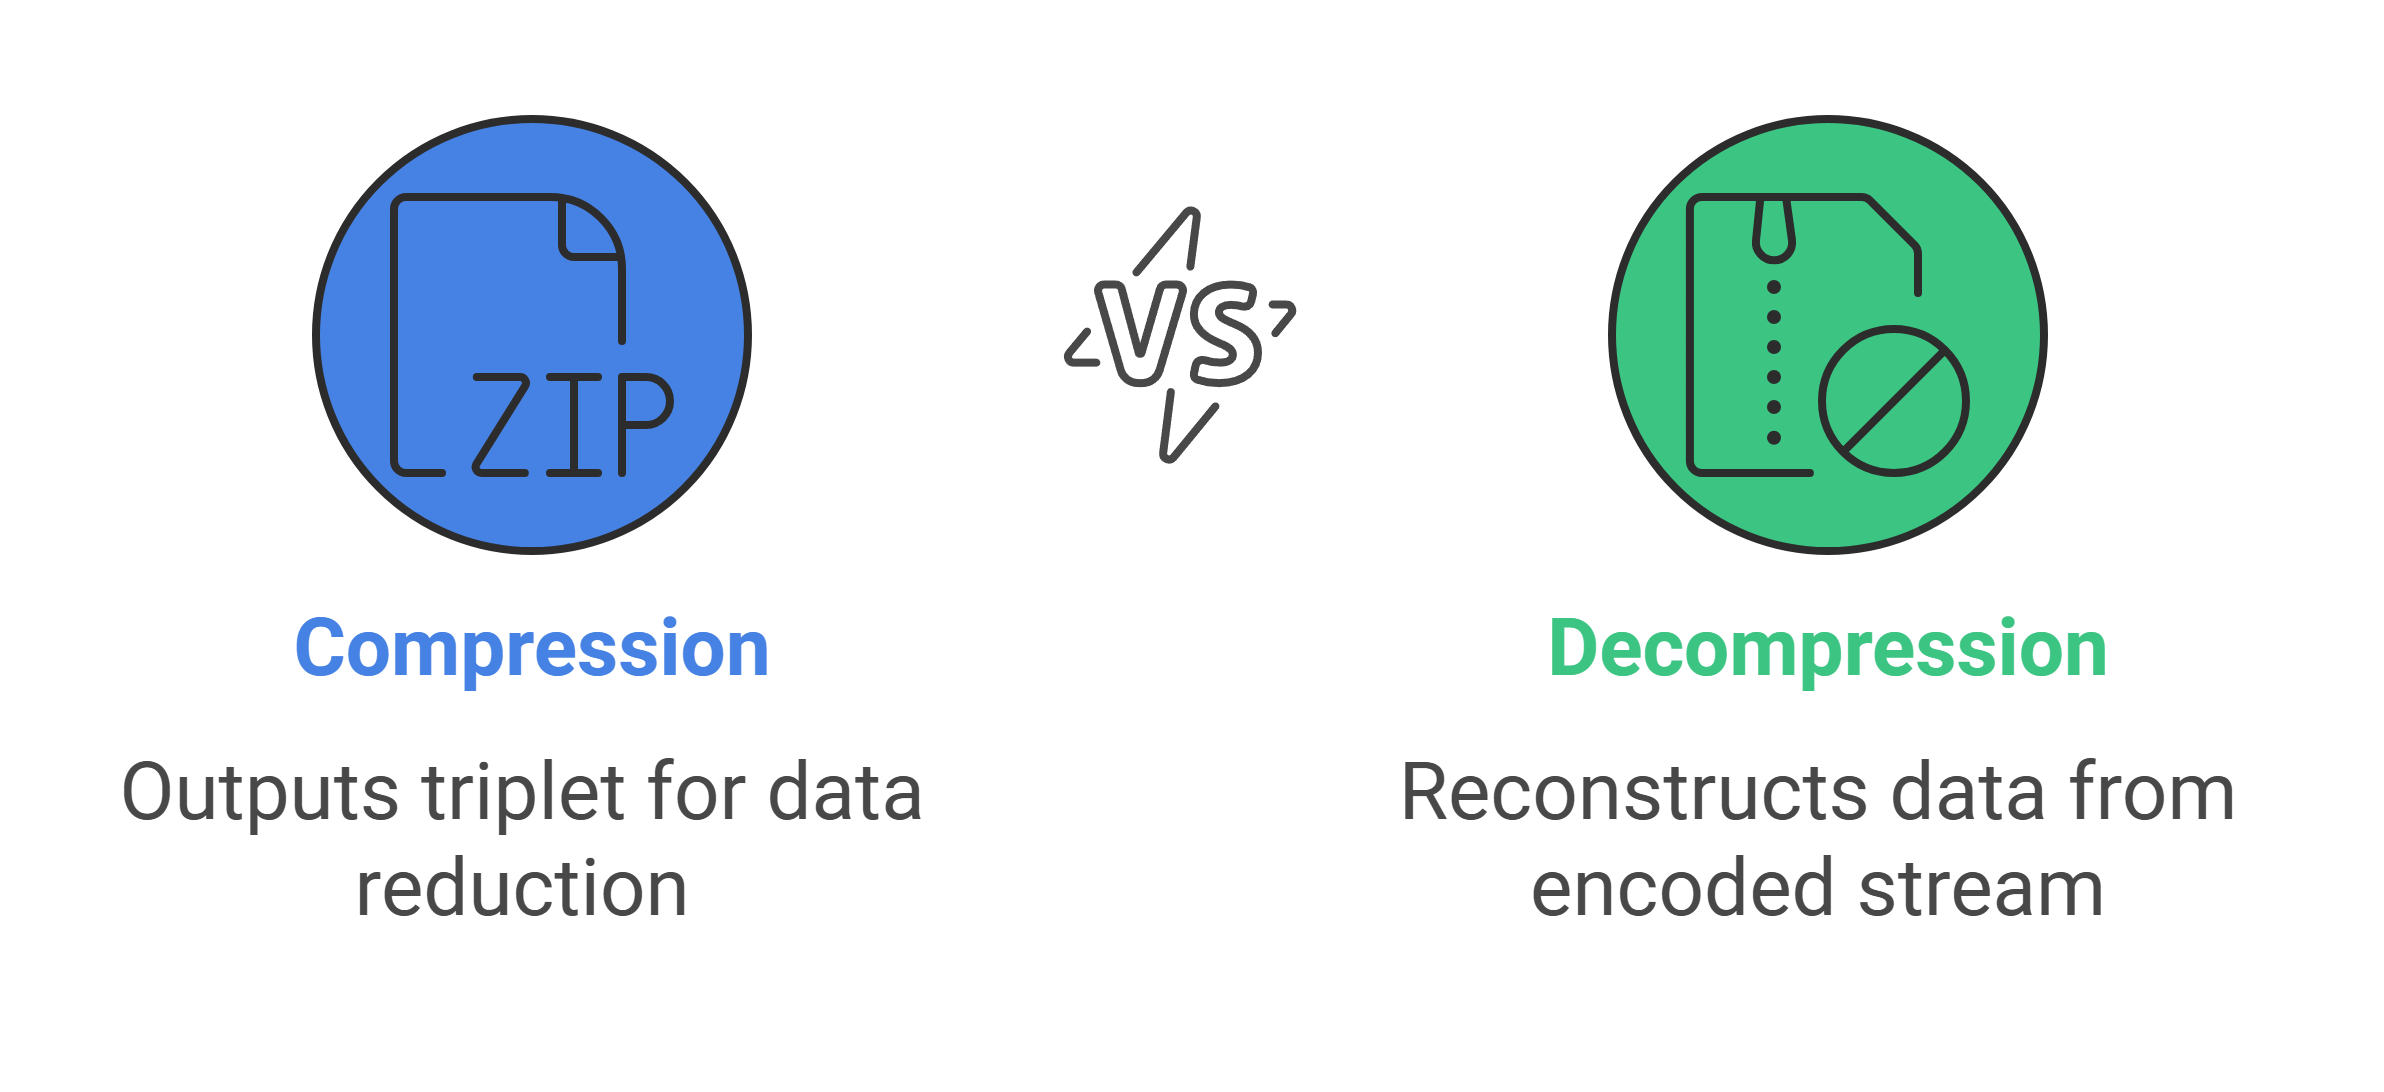
\includegraphics[width=0.8\linewidth]{Figures/LZ77.png}
    \caption{LZ77 Compression and Decompression}
    \label{fig:lz77}
\end{figure}

During compression, the algorithm outputs a triplet: a pointer to the starting position of the match (relative to the start of the sliding window), the length of the match, and the first unmatched character in the look-ahead buffer. If no match is found, the algorithm outputs a null pointer and the unmatched character.

\vspace{10pt}
% The decompression algorithm processes the compressed stream from start to end. For each null pointer, it appends the associated byte directly to the end of the output stream. For each non-null pointer, it reads back to the specified offset from the current end of the output stream and appends the specified number of bytes to the end of the output stream.

For decompression, the process starts by reading the encoded stream sequentially. When a null pointer is encountered, the algorithm appends the corresponding character to the output. For non-null pointers, the algorithm retrieves the matched substring using the pointer and length and then appends the retrieved substring to the output.

\subsection{LZ78}
% https://www.stringology.org/DataCompression/lz78/index_en.html#:~:text=Description,index%20instead%20of%20the%20phrase.
LZ78-based schemes work by entering phrases into a dictionary and then, when a repeat occurrence of that particular phrase is found, outputting the dictionary index instead of the phrase.

\begin{figure}[ht]
    \centering
    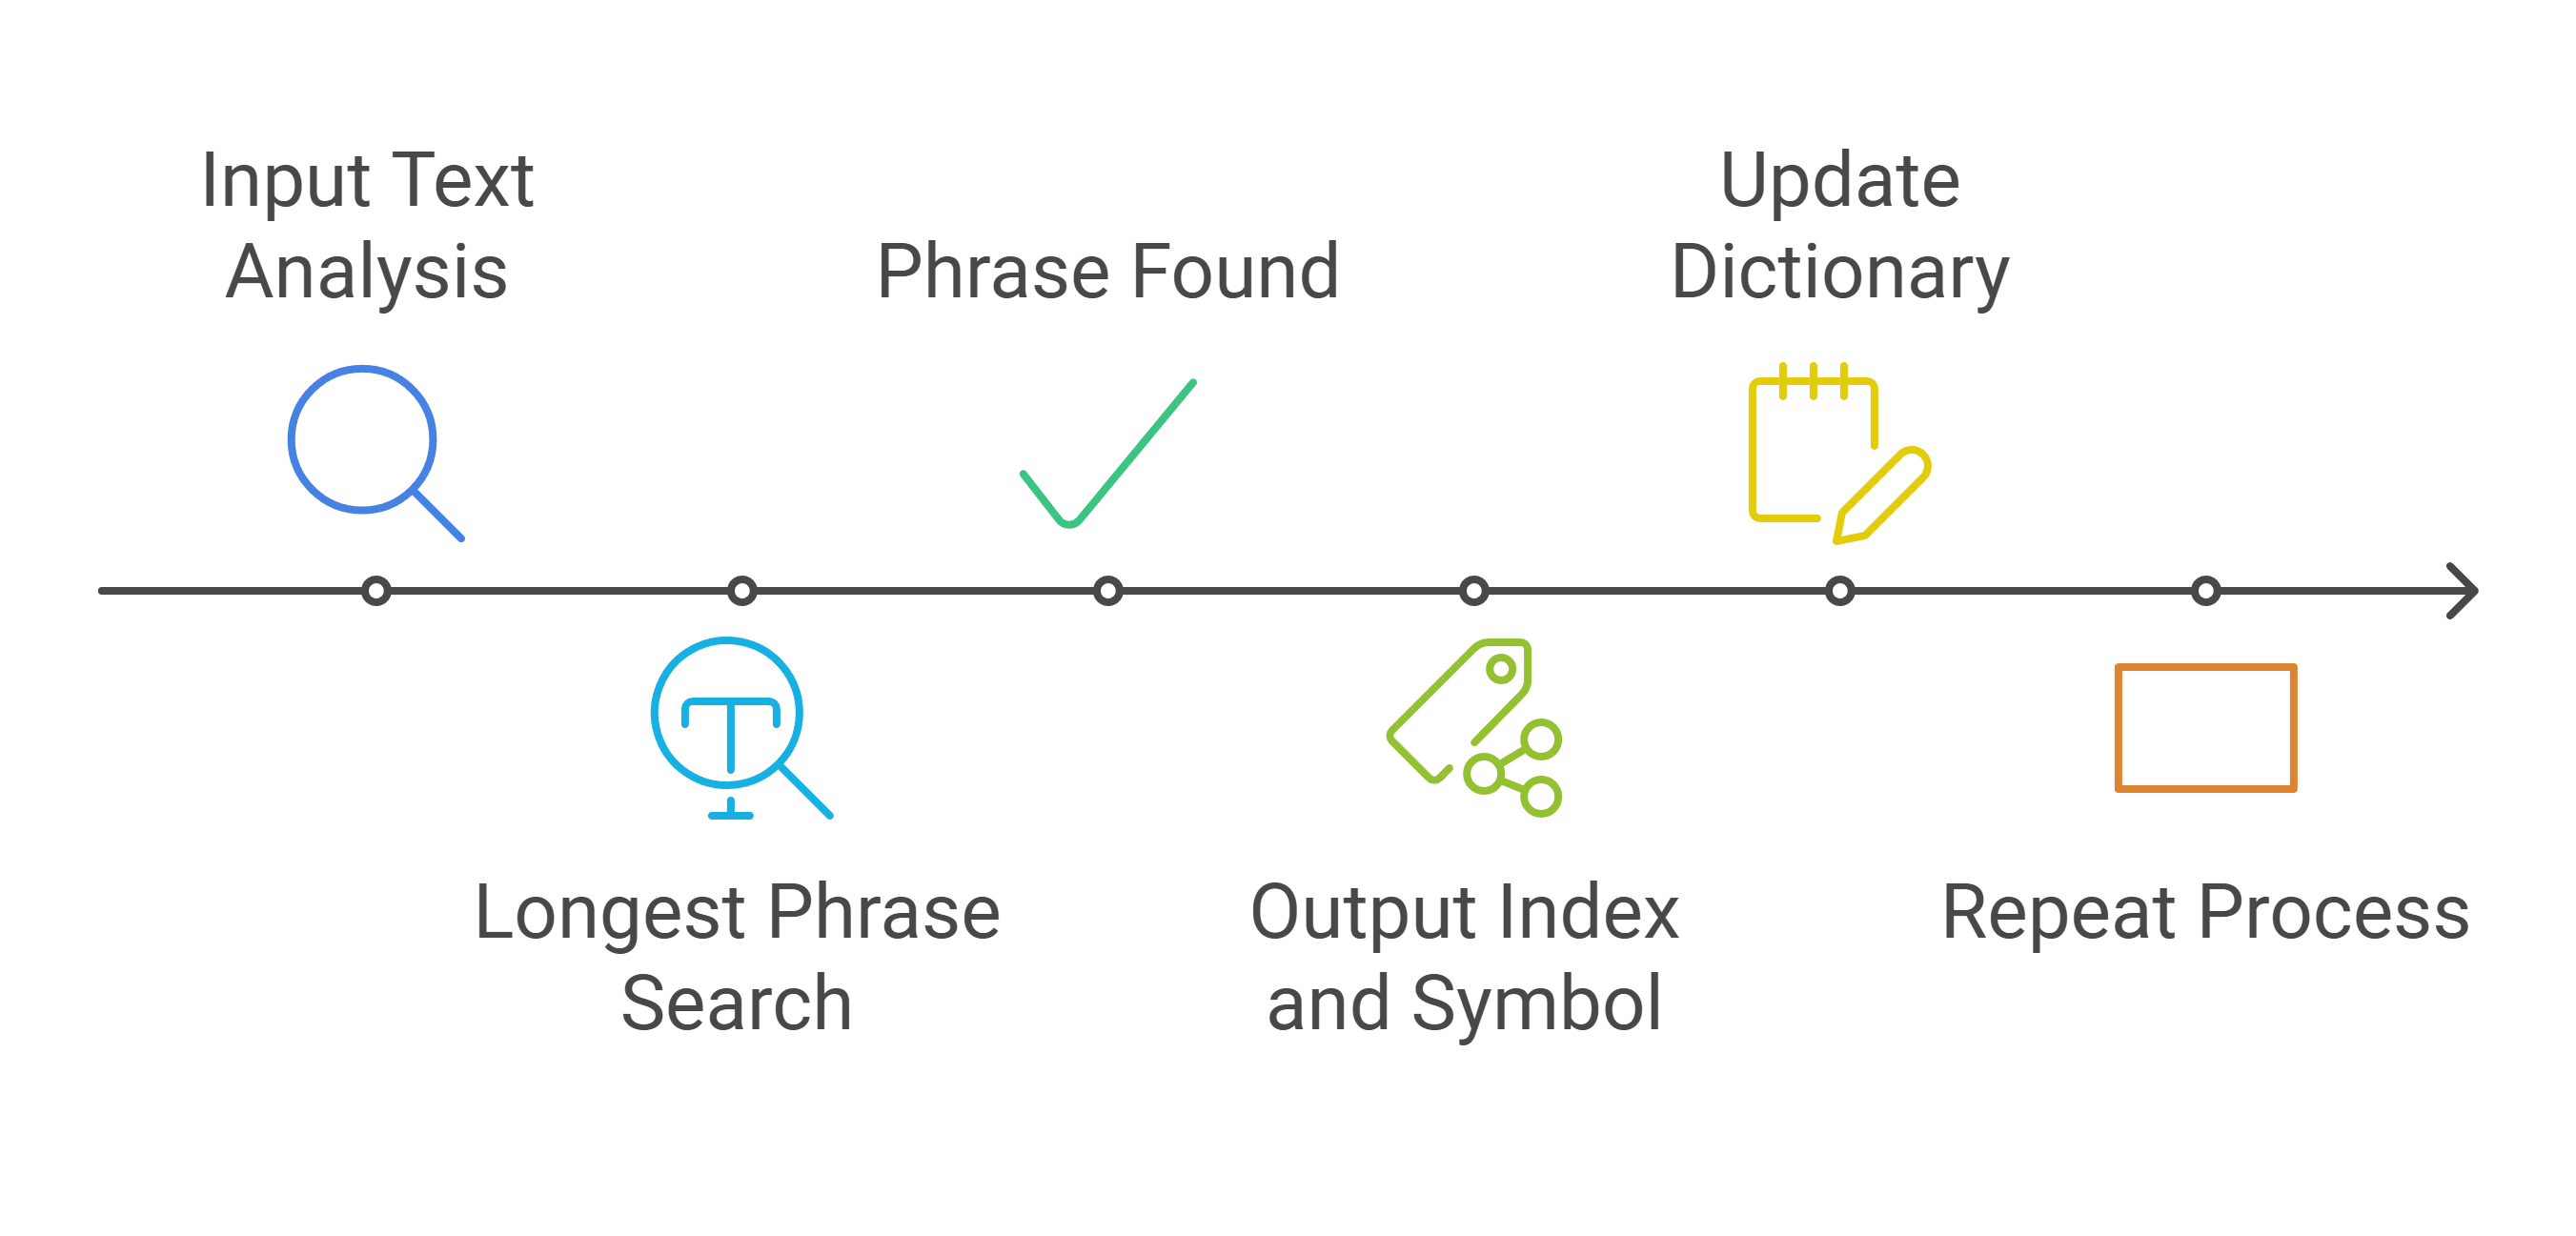
\includegraphics[width=1\linewidth]{Figures/LZ78.png}
    \caption{LZ78 Compression Process}
    \label{fig:lz78}
\end{figure}

At each step, LZ78\cite{doc5} outputs a pair (\textit{i, a}), where \textit{i} is the index of the phrase in the dictionary and \textit{a} is the next symbol following the phrase. The dictionary is represented like the trie with numbered nodes. If we go from the root to a certain node, we will get a phrase from the input text.

\vspace{10pt}
In each step, we look for the longest phrase in the dictionary, that would correspond to the unprocessed part of the input text. The index of this phrase together with the symbol, which follows the found part in the input text, is then sent to the output. The old phrase extended by the new symbol is then put into the dictionary. This new phrase is numbered by the smallest possible number.
\subsection{Comparison between LZ77, LZ78, and LZW}
LZ77, LZ78, and LZW are foundational compression algorithms that differ in their approach to handling redundancy in data. 

\vspace{10pt}

LZ77 operates using a sliding window, where it searches for the longest match between the look-ahead buffer (unprocessed data) and the sliding window (recently processed data). It outputs a triplet \textit{(offset, length, next symbol)}, with the offset indicating the starting position of the match, the length specifying the number of matched characters, and the next symbol representing the first unmatched character. This makes LZ77 effective for compressing data with localized repetition, but its performance diminishes when dealing with long-range patterns or globally repetitive data.

\vspace{10pt}

In contrast, LZ78 constructs an explicit and growing dictionary to store phrases dynamically as it processes the input. At each step, it outputs a pair \textit{(index, next symbol)}, where the index refers to the dictionary entry of the longest matching phrase, and the next symbol is the character that follows the match. Unlike LZ77, LZ78 does not limit itself to a sliding window, enabling it to capture patterns that recur over larger ranges in the input. However, the need to transmit the raw next symbol alongside the dictionary index can reduce compression efficiency for highly repetitive data.

\vspace{10pt}

LZW, an enhancement of LZ78, pre-initializes the dictionary with all single-character symbols, eliminating the need to transmit raw symbols in the output. This allows LZW to rely entirely on dictionary indices for encoding, which makes it more efficient than LZ78 for repetitive data. As the compression progresses, LZW extends the dictionary with new phrases formed from previously matched sequences. While this approach improves compression ratios for data with significant redundancy, it also introduces complexity in managing and synchronizing the dictionary between the encoder and decoder.

\vspace{10pt}

In terms of practical applications, LZ77 forms the basis of the widely used DEFLATE algorithm, which powers ZIP and PNG formats, with variants like LZSS optimizing its performance. LZ78 serves primarily as a theoretical foundation, influencing the development of algorithms like LZW, which gained widespread adoption in formats such as GIF. Each algorithm has its strengths: LZ77 excels with localized patterns, LZ78 handles long-range repetitions effectively, and LZW achieves high compression efficiency by using only dictionary indices. These differences make them suitable for various types of data and applications. 

\begin{table}[h!]
\caption{Comparison of LZ77, LZ78, and LZW.}
\centering
\begin{tabular}{|p{2.4cm}|p{4cm}|p{3.6cm}|p{4cm}|}
\hline
\textbf{Feature}            & \textbf{LZ77}                  & \textbf{LZ78}                  & \textbf{LZW}                  \\ \hline
\textbf{Dictionary Type}    & Sliding window                & Incremental, explicit trie     & Pre-initialized dictionary    \\ \hline
\textbf{Output}             & \((\text{offset, length, symbol})\) & \((\text{index, symbol})\)     & \((\text{index})\)            \\ \hline
\textbf{Strengths}          & Local repetition, flexibility & Long-range patterns            & High compression ratio        \\ \hline
\textbf{Weaknesses}         & Limited range                & Includes raw symbols           & Complex initialization        \\ \hline
\textbf{Applications}       & DEFLATE, ZIP, PNG            & Basis for LZW                  & GIF, legacy systems           \\ \hline
\end{tabular}
\label{tab:lz_comparison}
\end{table}

\newpage

% \section{Demonstrating Applications of LZW Compression}
% \subsection{Image Compression}
% \subsection{GIF Compression}
% \subsection{File Archiving}
% \subsection{Other Applications}
% \newpage

\section{Conclusion}
The Lempel-Ziv-Welch (LZW) algorithm, developed in 1984 by Abraham Lempel, Jakob Ziv, and Terry Welch, is a pivotal contribution to the field of lossless data compression. Renowned for its ability to efficiently reduce file sizes without losing information, LZW has become indispensable in various domains, including its prominent use in the GIF image format and the Unix compression utility compress.

\vspace{10pt}

As a dictionary-based compression algorithm, LZW optimizes storage and transmission by identifying repetitive patterns in the data and replacing them with shorter codes. This approach enables it to handle text, images, and other data types effectively, making it versatile for both general-purpose and specialized applications.

\vspace{10pt}

LZW's simplicity, efficiency, and adaptability have cemented its place as a foundational algorithm in computer science. Despite advancements in compression technology, LZW remains relevant, especially in legacy systems and formats where computational efficiency and lossless output are critical. Yet, its limitations highlight the need for selecting appropriate algorithms tailored to specific use cases.

\vspace{10pt}

In conclusion, the LZW algorithm is a testament to the power of innovative thinking in computer science, showcasing how efficient data representation can drive both technological and practical advancements in data storage and transmission.
\newpage

% \cleardoublepage
\phantomsection
\bibliographystyle{unsrt}
% \bibliography{ref/References}

\begin{thebibliography}{7}

\bibitem{doc1}
Jacob Ziv and Abraham Lempel, "Compression of individual sequences via variable-rate coding", \emph{IEEE Trans. Inf. Theory}, 24(5):530–536, 1978. Available: \url{https://api.semanticscholar.org/CorpusID:9267632}

\bibitem{doc2}
Terry A. Welch, "A technique for high-performance data compression", \emph{Computer},17(06):8–19, 1984. Available: \url{https://courses.cs.duke.edu/spring03/cps296.5/papers/welch_1984_technique_for.pdf}

\bibitem{doc3}
Jacob Ziv and Abraham Lempel, "A universal algorithm for sequential data compression", \emph{IEEE Transactions on Information Theory}, 23:337–343, 1977. 

\bibitem{doc4}
From Wikipedia, the free encyclopedia, "LZ77 and LZ78". Available: \url{https://en.wikipedia.org/wiki/LZ77_and_LZ78}

\bibitem{doc5}
From stringology.org, Czech Technical University in Prague, "Data Compression - LZ - 78". Available: \url{https://www.stringology.org/DataCompression/lz78/index_en.html}

\end{thebibliography}
\newpage

\section{Appendices}
\begin{longtable}{|>{\raggedright\arraybackslash}p{8.5cm}|>{\centering\arraybackslash}p{2.5cm}|>{\raggedright\arraybackslash}p{4cm}|}

\caption{Evaluation of Completion Rates for General Project Requirements}

% \hline
% \textbf{Requirement} & \textbf{Completion Rate (\%)} & \textbf{Remarks} \\ \hline
% \endfirsthead

\hline
\textbf{General Requirements} & \textbf{Completion Rate (\%)} & \textbf{Remarks} \\ \hline
\endhead
Group and member information (Student ID, full name, etc.) & 100 & Information provided completely and accurately. \\ \hline
Work assignment table, which includes information on each task assigned to team members, along with the completion rate of each member compared to the assigned tasks. & 100 & All tasks and contributions documented in detail. \\ \hline
Self-evaluation of the completion rate of the project requirements. & 100 & Honest and thorough self-assessment included. \\ \hline
Detailed description of each algorithm. Illustrative images and diagrams are encouraged. & 100 & Algorithms are well-explained with clear tables and examples. \\ \hline
Description of the test cases and experiment results along with your insights. & 100 & Test cases and results thoroughly analyzed with meaningful insights provided. \\ \hline
The report needs to be well-formatted and exported to PDF. If there are figures cut-off by the page break, etc., points will be deducted. & 100 & Formatting is clean and all figures are properly aligned without any cut-off. \\ \hline
References & 100 & Complete and correctly formatted reference list included. \\ \hline
\end{longtable}

\newpage

\begin{longtable}{|>{\raggedright\arraybackslash}p{8.5cm}|>{\centering\arraybackslash}p{2.5cm}|>{\raggedright\arraybackslash}p{4cm}|}

\caption{Evaluation of Completion Rates for Project LZW Compression Requirements}

% \hline
% \textbf{Requirement} & \textbf{Completion Rate (\%)} & \textbf{Remarks} \\ \hline
% \endfirsthead

\hline
\textbf{Requirements} & \textbf{Completion Rate (\%)} & \textbf{Remarks} \\ \hline
\endhead
Introduce its background: history and applications. & 100 & Background and applications of the algorithm are thoroughly explored, providing clear historical context and modern use cases. \\ \hline
Trace the algorithm, step by step, for both compression and decompression phases, using simple examples. & 100 & Step-by-step tracing includes clear examples for both phases, enhancing understanding. \\ \hline
Analyze the algorithm’s time complexity in the best case and worst case. & 100 & Comprehensive analysis provided with detailed calculations for both scenarios. \\ \hline
Present a comprehensive overview of LZW-related algorithms, such as the LZ77 and LZ78. For each algorithm, just give the overall idea while ignoring the details. & 100 & LZW-related algorithms are briefly but effectively summarized, focusing on key concepts. \\ \hline
\end{longtable}


\end{document}